\documentclass[xcolor=x11names, svgnames, rgb]{beamer}

\setbeamertemplate{navigation symbols}{}
\setbeamercolor{block title}{bg=blue!40}
\setbeamercolor{block body}{bg=blue!20}

%% Beamer Layout %%%%%%%%%%%%%%%%%%%%%%%%%%%%%%%%%%
\useoutertheme[subsection=false,shadow]{miniframes}
\useinnertheme{default}
\usefonttheme{serif}
\usepackage{palatino}
\setbeamerfont{title like}{shape=\scshape}
\setbeamerfont{frametitle}{shape=\scshape}
\setbeamercolor*{lower separation line head}{bg=DeepSkyBlue4}
\setbeamercolor*{normal text}{fg=black,bg=white}
\setbeamercolor*{alerted text}{fg=red}
\setbeamercolor*{example text}{fg=black}
\setbeamercolor*{structure}{fg=black}
\setbeamercolor*{palette tertiary}{fg=black,bg=black!10}
\setbeamercolor*{palette quaternary}{fg=black,bg=black!10}
%% END Beamer Layout %%%%%%%%%%%%%%%%%%%%%%%%%%%%%%%%%%%%%%%%%%%%
\usepackage{graphicx}
\usepackage{algpseudocode}

\usepackage{mathtools}
\newcommand{\defeq}{\vcentcolon=}
\DeclarePairedDelimiter{\paren}{(}{)}

\newcommand{\dec}{\operatorname{dec}}
\newcommand{\poly}{\operatorname{poly}}
\newcommand{\polylog}{\operatorname{polylog}}
\newcommand{\github}{\url{github.com/awestover/Parallel-Partition}}
\newcommand{\defn}[1]       {{\textit{\textbf{\boldmath #1}}}}
\newcommand{\paragraph}[1]{\vspace{0.09in}\noindent{\bf \boldmath #1.}} 
\usepackage{amsmath}
\def\E{\operatorname{\mathbb{E}}}
\usepackage{amssymb}
\usepackage{amsthm}

\newtheorem{proposition}{Proposition}
\newtheorem{defin}{Definition}

\usepackage{hyperref}

\usepackage{tikz,pgfplots}
\usepackage{etoolbox}
%% This makes the colors annoyingly bright, but at least they're easy to distinguish.
\pgfplotsset{
  every  tick/.style={red,}, minor x tick num=1,
  cycle list={teal,every mark/.append style={fill=teal!80!black},mark=*\\%
orange,every mark/.append style={fill=orange!80!black},mark=square*\\%
cyan!60!black,every mark/.append style={fill=cyan!80!black},mark=otimes*\\%
red!70!white,mark=star\\%
lime!80!black,every mark/.append style={fill=lime},mark=diamond*\\%
red,densely dashed,every mark/.append style={solid,fill=red!80!black},mark=*\\%
yellow!60!black,densely dashed,
every mark/.append style={solid,fill=yellow!80!black},mark=square*\\%
black,every mark/.append style={solid,fill=gray},mark=otimes*\\%
blue,densely dashed,mark=star,every mark/.append style=solid\\%
red,densely dashed,every mark/.append style={solid,fill=red!80!black},mark=diamond*\\%
}
}
\pgfplotsset{compat=1.6}

%% Issues: One }; missing in bandwidth table by default
%% Same issue appears multiple times in sort table

\def \CILKserialbaseline {3932.2}
\def \CILKblocksize {64}
\def \CILKnumtrials {5}
\def \CILKinputsize {1073741824}
\def \CILKtable {
\begin{tikzpicture}[scale = .8]
\begin{axis}[
width = 5 in,
height = 4in,
title={Speedup Over Serial Partition Versus Number of Threads},
xtick pos=left,
ytick pos=left,
legend style={draw=none},
axis line style = { draw = none },
legend pos= north west,
xtick = data,
xlabel={Number of Threads},
ylabel={Speedup Over Serial Partition},
ymax = 12,
legend columns = 2,
scatter/classes=%
{a={mark=o,draw=blue}}]
%% In-Place
\addplot coordinates {( 1, 0.499048) ( 2, 0.995494) ( 3, 1.42948) ( 4, 1.86113) ( 5, 2.26614) ( 6, 2.65797) ( 7, 2.97174) ( 8, 3.26921) ( 9, 3.43004) ( 10, 3.62281) ( 11, 3.78679) ( 12, 3.89481) ( 13, 4.0002) ( 14, 4.0986) ( 15, 4.15578) ( 16, 4.2191) ( 17, 4.22999) ( 18, 4.27599) };
%% In-Place Prefix-Sum
% \addplot coordinates {( 1, 0.35092) ( 2, 0.636608) ( 3, 0.894292) ( 4, 1.11755) ( 5, 1.32674) ( 6, 1.5096) ( 7, 1.65121) ( 8, 1.77494) ( 9, 1.88432) ( 10, 1.97837) ( 11, 2.0581) ( 12, 2.11591) ( 13, 2.15699) ( 14, 2.18845) ( 15, 2.21159) ( 16, 2.21657) ( 17, 2.20736) ( 18, 2.21557) };
%% Out-of-Place
\addplot coordinates {( 1, 0.223968) ( 2, 0.398625) ( 3, 0.551717) ( 4, 0.691607) ( 5, 0.812203) ( 6, 0.912936) ( 7, 0.990429) ( 8, 1.05055) ( 9, 1.09777) ( 10, 1.13562) ( 11, 1.15517) ( 12, 1.18848) ( 13, 1.20383) ( 14, 1.21364) ( 15, 1.22103) ( 16, 1.22575) ( 17, 1.22285) ( 18, 1.23444) };
%% %% High-Span
%% \addplot coordinates {( 1, 0.796443) ( 2, 1.58021) ( 3, 2.21882) ( 4, 2.93667) ( 5, 3.32899) ( 6, 3.80217) ( 7, 4.3662) ( 8, 4.93375) ( 9, 5.09881) ( 10, 5.42822) ( 11, 5.75051) ( 12, 6.01806) ( 13, 6.37103) ( 14, 6.57999) ( 15, 6.72631) ( 16, 6.95718) ( 17, 7.06722) ( 18, 7.34442) };
%% Cache-Friendly
\addplot coordinates {( 1, 0.619888) ( 2, 1.24099) ( 3, 1.80558) ( 4, 2.38286) ( 5, 2.95654) ( 6, 3.52917) ( 7, 4.09348) ( 8, 4.63922) ( 9, 5.19034) ( 10, 5.72539) ( 11, 6.27145) ( 12, 6.80311) ( 13, 7.34442) ( 14, 7.85497) ( 15, 8.24706) ( 16, 8.57062) ( 17, 8.77723) ( 18, 9.5674) };
%% Strided
\addplot coordinates {( 1, 0.767408) ( 2, 1.5359) ( 3, 2.21084) ( 4, 2.89005) ( 5, 3.56954) ( 6, 4.2382) ( 7, 4.9214) ( 8, 5.58393) ( 9, 6.23961) ( 10, 6.90587) ( 11, 7.54451) ( 12, 8.18186) ( 13, 8.83243) ( 14, 9.4207) ( 15, 9.88984) ( 16, 10.3425) ( 17, 10.4524) ( 18, 11.1205) };
\legend{Kuszmaul's In-Place, Standard Linear-Space, Smoothed-Striding, Strided} %% Low-Space, Med-Space, High-Space, Smoothed-Striding, Strided 
\end{axis}
\end{tikzpicture}
}
\def \partitionbandwidthboundserialbaseline {3933.6}
\def \partitionbandwidthboundblocksize {64}
\def \partitionbandwidthboundnumtrials {5}
\def \partitionbandwidthboundinputsize {1073741824}
\def \partitionbandwidthboundtable {
\begin{tikzpicture}[scale = .8]
\begin{axis}[
width = 5 in,
height = 4in,
title={Speedup Over Serial Partition and Bandwidth Constraint Versus Number of Threads},
xtick pos=left,
ytick pos=left,
legend style={draw=none},
axis line style = { draw = none },
legend pos= north west,
xtick = data,
xlabel={Number of Threads},
ylabel={Speedup Over Serial Partition},
ymax = 20,
legend columns = 2,
scatter/classes=%
{a={mark=o,draw=blue}}]
%% In-Place
\addplot coordinates {( 1, 0.499378) ( 2, 0.995949) ( 3, 1.4328) ( 4, 1.86816) ( 5, 2.26982) ( 6, 2.66432) ( 7, 2.98407) ( 8, 3.26602) ( 9, 3.43066) ( 10, 3.61544) ( 11, 3.79325) ( 12, 3.91949) ( 13, 4.00244) ( 14, 4.08389) ( 15, 4.15375) ( 16, 4.22151) ( 17, 4.25438) ( 18, 4.25622) };
%% Low-Space Bandwidth Bound
\addplot coordinates {(1, 0.894939)(2, 1.72634)(3, 2.26699)(4, 2.66131)(5, 3.15777)(6, 3.4024)(7, 3.50312)(8, 3.49686)(9, 3.62955)(10, 3.74294)(11, 3.90093)(12, 3.9593)(13, 4.0131)(14, 4.04714)(15, 4.13799)(16, 4.13782)(17, 4.10515)(18, 4.15355)};
%% high span
%% \addplot coordinates {( 1, 0.812828) ( 2, 1.61997) ( 3, 2.22137) ( 4, 2.95626) ( 5, 3.33582) ( 6, 3.80352) ( 7, 4.36001) ( 8, 5.10062) ( 9, 5.11521) ( 10, 5.44217) ( 11, 5.74752) ( 12, 6.07787) ( 13, 6.41278) ( 14, 6.63787) ( 15, 6.68752) ( 16, 6.79848) ( 17, 7.10549) ( 18, 7.26292) };
%% %% High-Span Bandwidth Bound
%% \addplot coordinates {(1, 1.75849)(2, 3.34185)(3, 4.35383)(4, 5.15739)(5, 5.9788)(6, 6.31621)(7, 6.76074)(8, 6.76348)(9, 6.99773)(10, 7.10173)(11, 7.39957)(12, 7.51437)(13, 7.7436)(14, 7.76191)(15, 7.89966)(16, 7.87403)(17, 7.94484)(18, 8.05483)}; %% cache friendly
\addplot coordinates {( 1, 0.62101) ( 2, 1.24639) ( 3, 1.81072) ( 4, 2.37852) ( 5, 2.95182) ( 6, 3.53233) ( 7, 4.09153) ( 8, 4.63759) ( 9, 5.18124) ( 10, 5.73746) ( 11, 6.27769) ( 12, 6.82206) ( 13, 7.35802) ( 14, 7.81717) ( 15, 8.17117) ( 16, 8.81183) ( 17, 8.81973) ( 18, 9.18636) };
%% Cache-Friendly Bandwidth Bound
\addplot coordinates {(1, 3.52223)(2, 6.68603)(3, 8.70095)(4, 10.276)(5, 12.1258)(6, 12.8292)(7, 13.4991)(8, 13.4622)(9, 14.1134)(10, 14.1066)(11, 14.8215)(12, 15.3338)(13, 15.3938)(14, 15.3942)(15, 15.8412)(16, 15.5877)(17, 15.9778)(18, 15.9519)};
\legend{Kuszmaul's In-Place, Kuszmaul's In-Place Bandwidth Constraint, Smoothed Striding, Smoothed Striding Bandwidth Constraint}
\end{axis}
\end{tikzpicture}
}

\def \CILKsortblocksize {64}
\def \CILKsortnumtrials {5}
\def \CILKsortmaxinputsize {1073741824}
\def \CILKsorttable {
\begin{tikzpicture}[scale = .8]
\begin{axis}[
width = 5 in,
height = 4in,
title={Speedup Of Quicksort Over Serial Partition's Quicksort Versus Number of Threads},
xtick pos=left,
ytick pos=left,
legend style={draw=none},
axis line style = { draw = none },
legend pos= north west,
xtick = data,
xlabel={Number of Threads},
ylabel={Speedup Over Serial Partition},
ymax = 15,
legend columns = 2,
scatter/classes=%
{a={mark=o,draw=blue}}]
%% %% Low Space with log size 24
%% \addplot coordinates {( 1, 0.863202) ( 2, 1.63232) ( 3, 2.29705) ( 4, 2.96413) ( 5, 3.59298) ( 6, 4.1696) ( 7, 4.71085) ( 8, 5.2279) ( 9, 5.8474) ( 10, 6.4043) ( 11, 6.55736) ( 12, 7.21241) ( 13, 7.57064) ( 14, 7.99417) ( 15, 8.4679) ( 16, 8.93099) ( 17, 9.04881) ( 18, 9.60644) %% High-Span with log size 24
%% \addplot coordinates {( 1, 0.960106) ( 2, 1.88538) ( 3, 2.72075) ( 4, 3.47467) ( 5, 4.2576) ( 6, 5.08451) ( 7, 5.93339) ( 8, 6.47686) ( 9, 7.1822) ( 10, 7.57901) ( 11, 8.44704) ( 12, 8.64943) ( 13, 9.16979) ( 14, 9.04881) ( 15, 10.1464) ( 16, 9.61992) ( 17, 10.5199) ( 18, 9.38304) %% Cache Friendly with log size 24
%% \addplot coordinates {( 1, 0.900013) ( 2, 1.74752) ( 3, 2.46372) ( 4, 3.23233) ( 5, 3.90159) ( 6, 4.62508) ( 7, 5.46099) ( 8, 6.15157) ( 9, 6.85215) ( 10, 7.53736) ( 11, 8.11716) ( 12, 8.74872) ( 13, 9.70156) ( 14, 9.04881) ( 15, 11.0273) ( 16, 10.87) ( 17, 12.1829) ( 18, 12.2482) %% Strided with log size 24
%% \addplot coordinates {( 1, 0.95079) ( 2, 1.82955) ( 3, 2.63808) ( 4, 3.45716) ( 5, 4.20798) ( 6, 4.99199) ( 7, 5.78819) ( 8, 6.56364) ( 9, 7.37527) ( 10, 8.03162) ( 11, 8.89624) ( 12, 9.61992) ( 13, 9.7153) ( 14, 11.1167) ( 15, 10.9394) ( 16, 11.4891) ( 17, 13.1651) ( 18, 13.9695) };
%% %% Low Space with log size 26
%% \addplot coordinates {( 1, 0.861043) ( 2, 1.63325) ( 3, 2.3004) ( 4, 2.98343) ( 5, 3.63316) ( 6, 4.19898) ( 7, 4.82886) ( 8, 5.34581) ( 9, 5.89992) ( 10, 6.44372) ( 11, 6.94206) ( 12, 7.4672) ( 13, 7.60676) ( 14, 8.0564) ( 15, 8.64475) ( 16, 8.82709) ( 17, 8.76202) ( 18, 8.96831) %% High-Span with log size 26
%% \addplot coordinates {( 1, 0.955523) ( 2, 1.86586) ( 3, 2.6845) ( 4, 3.49224) ( 5, 4.27081) ( 6, 5.0929) ( 7, 5.83274) ( 8, 6.53586) ( 9, 7.29308) ( 10, 7.90003) ( 11, 8.63721) ( 12, 8.97915) ( 13, 9.7769) ( 14, 10.1893) ( 15, 10.5812) ( 16, 10.7887) ( 17, 10.7613) ( 18, 10.3418) %% Cache Friendly with log size 26
%% \addplot coordinates {( 1, 0.914609) ( 2, 1.73339) ( 3, 2.49178) ( 4, 3.22151) ( 5, 4.02384) ( 6, 4.70946) ( 7, 5.57239) ( 8, 6.13884) ( 9, 6.93881) ( 10, 7.59315) ( 11, 8.23047) ( 12, 8.91717) ( 13, 9.42939) ( 14, 10.1302) ( 15, 10.6801) ( 16, 10.8359) ( 17, 11.3883) ( 18, 11.3189) %% Strided with log size 26
%% \addplot coordinates {( 1, 0.946785) ( 2, 1.82922) ( 3, 2.64766) ( 4, 3.4262) ( 5, 4.2788) ( 6, 5.08245) ( 7, 5.95192) ( 8, 6.67986) ( 9, 7.44475) ( 10, 8.25563) ( 11, 8.94132) ( 12, 9.74164) ( 13, 10.4362) ( 14, 11.3621) ( 15, 11.4851) ( 16, 12.2071) ( 17, 12.6542) ( 18, 13.4993) };
%% %% Low Space with log size 28
%% \addplot coordinates {( 1, 0.862267) ( 2, 1.63941) ( 3, 2.34664) ( 4, 2.96157) ( 5, 3.64611) ( 6, 4.31258) ( 7, 4.88345) ( 8, 5.43042) ( 9, 5.87762) ( 10, 6.44029) ( 11, 7.00878) ( 12, 7.30452) ( 13, 7.83539) ( 14, 8.12956) ( 15, 8.50856) ( 16, 8.76302) ( 17, 8.98741) ( 18, 9.33821) %% High-Span with log size 28
%% \addplot coordinates {( 1, 0.939362) ( 2, 1.84744) ( 3, 2.6917) ( 4, 3.45716) ( 5, 4.29244) ( 6, 5.08279) ( 7, 5.79208) ( 8, 6.6353) ( 9, 7.2093) ( 10, 8.01682) ( 11, 8.74742) ( 12, 9.17326) ( 13, 9.7479) ( 14, 10.2979) ( 15, 11.0745) ( 16, 11.4344) ( 17, 11.4888) ( 18, 12.34) %% Cache Friendly with log size 28
%% \addplot coordinates {( 1, 0.908881) ( 2, 1.75263) ( 3, 2.51771) ( 4, 3.28228) ( 5, 4.01042) ( 6, 4.74982) ( 7, 5.54834) ( 8, 6.2393) ( 9, 6.98884) ( 10, 7.70125) ( 11, 8.41219) ( 12, 9.06778) ( 13, 9.67555) ( 14, 10.3505) ( 15, 11.0125) ( 16, 11.4744) ( 17, 12.1533) ( 18, 12.4095) %% Strided with log size 28
%% \addplot coordinates {( 1, 0.942529) ( 2, 1.82563) ( 3, 2.6044) ( 4, 3.46053) ( 5, 4.25683) ( 6, 5.12315) ( 7, 5.88602) ( 8, 6.70811) ( 9, 7.43113) ( 10, 8.17952) ( 11, 8.96974) ( 12, 9.68435) ( 13, 10.4214) ( 14, 10.9587) ( 15, 11.71) ( 16, 12.2949) ( 17, 12.9046) ( 18, 13.3107) };
%% Low Space with log size 30
\addplot coordinates {( 1, 0.87864) ( 2, 1.68661) ( 3, 2.39404) ( 4, 3.03172) ( 5, 3.71549) ( 6, 4.45118) ( 7, 5.07595) ( 8, 5.76618) ( 9, 6.26716) ( 10, 6.79929) ( 11, 7.34223) ( 12, 7.74736) ( 13, 8.17148) ( 14, 8.70784) ( 15, 8.91736) ( 16, 9.26139) ( 17, 9.47532) ( 18, 9.68665)}; %% High-Span with log size 30
%% \addplot coordinates {( 1, 0.96225) ( 2, 1.879) ( 3, 2.71741) ( 4, 3.56118) ( 5, 4.44821) ( 6, 5.29223) ( 7, 5.97895) ( 8, 6.76091) ( 9, 7.59373) ( 10, 8.37912) ( 11, 9.01587) ( 12, 9.58729) ( 13, 10.1906) ( 14, 10.881) ( 15, 11.4166) ( 16, 12.026) ( 17, 12.3279) ( 18, 12.6408)}; %% Cache Friendly with log size 30
\addplot coordinates {( 1, 0.921182) ( 2, 1.80562) ( 3, 2.57745) ( 4, 3.37831) ( 5, 4.15358) ( 6, 4.91613) ( 7, 5.7093) ( 8, 6.41041) ( 9, 7.14098) ( 10, 7.907) ( 11, 8.6573) ( 12, 9.46479) ( 13, 10.1098) ( 14, 10.7975) ( 15, 11.4046) ( 16, 12.1549) ( 17, 12.7427) ( 18, 13.346)}; %% Strided with log size 30
\addplot coordinates {( 1, 0.949951) ( 2, 1.87888) ( 3, 2.70758) ( 4, 3.52248) ( 5, 4.40049) ( 6, 5.19675) ( 7, 6.02708) ( 8, 6.79362) ( 9, 7.69896) ( 10, 8.36354) ( 11, 9.17828) ( 12, 9.92823) ( 13, 10.7114) ( 14, 11.4187) ( 15, 12.0935) ( 16, 12.8171) ( 17, 13.5719) ( 18, 14.2507) };
\legend{Kuszmaul's In-Place, Smoothed Striding, Strided}
\end{axis}
\end{tikzpicture}
}

%% Bandwith results without numactl:
%% \def \partitionbandwidthboundserialbaseline {3832}
%% \def \partitionbandwidthboundblocksize {64}
%% \def \partitionbandwidthboundnumtrials {5}
%% \def \partitionbandwidthboundinputsize {1073741824}
%% \def \partitionbandwidthboundtable {
%% \begin{tikzpicture}[scale = .8]
%% \begin{axis}[
%% width = 5 in,
%% height = 4in,
%% title={Speedup Versus Number of Threads},
%% xtick pos=left,
%% ytick pos=left,
%% legend style={draw=none},
%% axis line style = { draw = none },
%% legend pos= north west,
%% xtick = data,
%% xlabel={Number of Threads},
%% ylabel={Speedup Over Serial Partition},
%% ymax = 4,
%% legend columns = 2,
%% scatter/classes=%
%% {a={mark=o,draw=blue}}]
%% %% In-Place
%% \addplot coordinates {( 1, 0.504928) ( 2, 0.744917) ( 3, 1.27793) ( 4, 1.62967) ( 5, 1.91677) ( 6, 2.3244) ( 7, 2.47865) ( 8, 2.58186) ( 9, 2.68573) ( 10, 2.78448) ( 11, 2.7756) ( 12, 2.85077) ( 13, 2.86826) ( 14, 2.91407) ( 15, 2.90479) ( 16, 2.94769) ( 17, 2.95497) ( 18, 2.94588) };
%% %% Low-Space Bandwidth Bound
%% \addplot coordinates {(1, 1.05385)(2, 1.63936)(3, 1.81183)(4, 2.05614)(5, 2.39067)(6, 2.5237)(7, 2.40513)(8, 2.55015)(9, 2.58884)(10, 2.57444)(11, 2.69167)(12, 2.66946)(13, 2.64859)(14, 2.68175)(15, 2.66023)(16, 2.69318)(17, 2.68783)(18, 2.72913)};
%% %% high span
%% \addplot coordinates {( 1, 0.816814) ( 2, 1.47691) ( 3, 1.98529) ( 4, 2.63875) ( 5, 3.01305) ( 6, 3.40441) ( 7, 3.68887) ( 8, 3.97345) ( 9, 4.14181) ( 10, 4.27297) ( 11, 4.46724) ( 12, 4.45271) ( 13, 4.45271) ( 14, 4.62355) ( 15, 4.60024) ( 16, 4.70184) ( 17, 4.55431) ( 18, 4.71225) };
%% %% High-Span Bandwidth Bound
%% \addplot coordinates {(1, 2.03744)(2, 3.14521)(3, 3.47353)(4, 3.91661)(5, 4.536)(6, 4.70395)(7, 4.47075)(8, 4.76355)(9, 4.86065)(10, 4.68934)(11, 4.86418)(12, 4.98468)(13, 4.9239)(14, 4.99117)(15, 4.94174)(16, 4.98761)(17, 4.96382)(18, 5.00564)%% cache friendly
%% \addplot coordinates {( 1, 0.621291) ( 2, 1.06581) ( 3, 1.76541) ( 4, 2.28204) ( 5, 2.8838) ( 6, 3.49253) ( 7, 4.04561) ( 8, 4.56843) ( 9, 4.97921) ( 10, 5.6089) ( 11, 5.8791) ( 12, 6.26963) ( 13, 6.8331) ( 14, 6.87971) ( 15, 7.15459) ( 16, 7.38343) ( 17, 8.25151) ( 18, 8.35587) };
%% %% Cache-Friendly Bandwidth Bound
%% \addplot coordinates {(1, 4.06363)(2, 6.29023)(3, 6.9299)(4, 7.88794)(5, 9.08502)(6, 9.329)(7, 9.45987)(8, 9.53406)(9, 9.91163)(10, 9.90729)(11, 9.70433)(12, 10.1146)(13, 9.9126)(14, 9.85886)(15, 9.86993)(16, 10.0183)(17, 10.0765)(18, 9.99261)};
%% \legend{Low-Space, Low-Space Bandwidth Constraint, Two-Layer, Two-Layer Bandwidth Constraint}
%% \end{axis}
%% \end{tikzpicture}
%% }

\def \serialnumtrials {5}
\def \serialblocksize {64}
\def \serialtable {
\begin{tikzpicture}[scale = .8]
\begin{axis}[
width = 5 in,
height = 4in,
title={Slowdown Over Serial Partition Versus Input Size in Serial},
xtick pos=left,
ytick pos=left,
ymax = 6,
ymin = 0,
legend style={draw=none},
axis line style = { draw = none },
legend pos= north west,
xtick = data,
xlabel={Log Input Size},
ylabel={Slowdown Over Serial Partition},
legend columns = 2,
scatter/classes=%
{a={mark=o,draw=blue}}]
%% Serial Baseline
%% baselines in ms: \addplot coordinates {( 23, 30.4 ) ( 24, 61 ) ( 25, 122.4 ) ( 26, 244.8 ) ( 27, 489.6 ) ( 28, 979.6 ) ( 29, 1963.4 ) ( 30, 3922.6 ) };
%% In-Place
\addplot coordinates {( 23, 1.82895) ( 24, 1.81639) ( 25, 1.83007) ( 26, 1.83905) ( 27, 1.84722) ( 28, 1.89343) ( 29, 1.90068) ( 30, 1.91837) };
%% In-Place Prefix-Sum
% \addplot coordinates {( 23, 2.75658) ( 24, 2.71803) ( 25, 2.68137) ( 26, 2.67157) ( 27, 2.67443) ( 28, 2.70131) ( 29, 2.70551) ( 30, 2.71713) };
%% Out-of-Place
\addplot coordinates {( 23, 4.31579) ( 24, 4.26885) ( 25, 4.20098) ( 26, 4.18464) ( 27, 4.18546) ( 28, 4.22519) ( 29, 4.22257) ( 30, 4.23265) };
%% %% High-Span
%% \addplot coordinates {( 23, 1.23684) ( 24, 1.23934) ( 25, 1.24346) ( 26, 1.24428) ( 27, 1.24632) ( 28, 1.24602) ( 29, 1.24417) ( 30, 1.2456) };
%% Cache-Friendly
\addplot coordinates {( 23, 1.55263) ( 24, 1.54426) ( 25, 1.53431) ( 26, 1.53431) ( 27, 1.53554) ( 28, 1.53491) ( 29, 1.55852) ( 30, 1.53317) };
%% Strided
\addplot coordinates {( 23, 1.53289) ( 24, 1.53443) ( 25, 1.53105) ( 26, 1.52778) ( 27, 1.53064) ( 28, 1.52613) ( 29, 1.5246) ( 30, 1.52919) };
\legend{Kuszmaul's In-Place, Standard Linear-Space, Smoothed Striding, Strided} % Low-Space, Med-Space, High-Space, Smoothed Striding, Strided
\end{axis}
\end{tikzpicture}
}
%% \def \serialnumtrials {5}
%% \def \serialblocksize {64}
%% \def \serialtable {
%% \begin{tikzpicture}[scale = .8]
%% \begin{axis}[
%% width = 5 in,
%% height = 4in,
%% title={Slowdown Versus Input Size in Serial},
%% xtick pos=left,
%% ytick pos=left,
%% ymax = 5,
%% ymin = 0,
%% legend style={draw=none},
%% axis line style = { draw = none },
%% legend pos= north west,
%% xtick = data,
%% xlabel={Log Input Size},
%% ylabel={Slowdown Over Serial Partition},
%% legend columns = 2,
%% scatter/classes=%
%% {a={mark=o,draw=blue}}]
%% %% Serial Baseline
%% %% baselines in ms: \addplot coordinates {( 23, 30.4 ) ( 24, 61 ) ( 25, 122.4 ) ( 26, 244.8 ) ( 27, 489.6 ) ( 28, 979.6 ) ( 29, 1963.4 ) ( 30, 3922.6 ) };
%% %% In-Place
%% \addplot coordinates {( 23, 1.82895) ( 24, 1.81639) ( 25, 1.83007) ( 26, 1.83905) ( 27, 1.84722) ( 28, 1.89343) ( 29, 1.90068) ( 30, 1.91837) };
%% %% In-Place Prefix-Sum
%% \addplot coordinates {( 23, 2.75658) ( 24, 2.71803) ( 25, 2.68137) ( 26, 2.67157) ( 27, 2.67443) ( 28, 2.70131) ( 29, 2.70551) ( 30, 2.71713) };
%% %% Out-of-Place
%% \addplot coordinates {( 23, 4.31579) ( 24, 4.26885) ( 25, 4.20098) ( 26, 4.18464) ( 27, 4.18546) ( 28, 4.22519) ( 29, 4.22257) ( 30, 4.23265) };
%% %% High-Span
%% \addplot coordinates {( 23, 1.23684) ( 24, 1.23934) ( 25, 1.24346) ( 26, 1.24428) ( 27, 1.24632) ( 28, 1.24602) ( 29, 1.24417) ( 30, 1.2456) };
%% %% Cache-Friendly
%% \addplot coordinates {( 23, 1.55263) ( 24, 1.54426) ( 25, 1.53431) ( 26, 1.53431) ( 27, 1.53554) ( 28, 1.53491) ( 29, 1.55852) ( 30, 1.53317) };
%% %% Strided
%% \addplot coordinates {( 23, 1.53289) ( 24, 1.53443) ( 25, 1.53105) ( 26, 1.52778) ( 27, 1.53064) ( 28, 1.52613) ( 29, 1.5246) ( 30, 1.52919) };
%% \legend{Low-Space, Med-Space, High-Space, Two-Layer, Cache-Friendly, Strided}
%% \end{axis}
%% \end{tikzpicture}
%% }
%% \def \serialnumtrials {1}
%% \def \serialblocksize {64}
%% \def \serialtable {
%% \begin{tikzpicture}[scale = .8]
%% \begin{axis}[
%% title={Slowdown Versus Input Size in Serial},
%% width = 5in, %%!!!!
%% height = 4in,
%% xtick pos=left,
%% ytick pos=left,
%% ymax = 5, %% !!!
%% ymin = 0,
%% legend style={draw=none},
%% axis line style = { draw = none },
%% legend pos= north west,
%% xtick = data,
%% xlabel={Log Input Size},
%% ylabel={Slowdown Over Serial Partition},
%% legend columns = 2,
%% scatter/classes=%
%% {a={mark=o,draw=blue}}]
%% %% Serial Baseline%% baselines in ms: \addplot coordinates {( 23, 30.4 ) ( 24, 60.8 ) ( 25, 121.4 ) ( 26, 243.8 ) ( 27, 487.4 ) ( 28, 975.8 ) ( 29, 1952.2 ) ( 30, 3902 ) };
%% %% In-Place
%% \addplot coordinates {( 23, 1.79605) ( 24, 1.82237) ( 25, 1.84185) ( 26, 1.84249) ( 27, 1.87033) ( 28, 1.90838) ( 29, 1.90687) ( 30, 1.91579) };
%% %% In-Place Prefix-Sum
%% \addplot coordinates {( 23, 2.58553) ( 24, 2.57237) ( 25, 2.57661) ( 26, 2.56932) ( 27, 2.56422) ( 28, 2.59459) ( 29, 2.60834) ( 30, 2.61107) };
%% %% Out-of-Place
%% \addplot coordinates {( 23, 3.98684) ( 24, 3.96711) ( 25, 3.96705) ( 26, 3.96308) ( 27, 3.98195) ( 28, 4.01537) ( 29, 4.03401) ( 30, 4.06079) };
%% %% High-Span
%% \addplot coordinates {( 23, 1.21053) ( 24, 1.23355) ( 25, 1.23558) ( 26, 1.23298) ( 27, 1.23677) ( 28, 1.24124) ( 29, 1.24096) ( 30, 1.23931) };
%% \legend{Low-Space, Med-Space, High-Space, Two-Layer} %% Two-layer instead of high-span everywhere
%% \end{axis}
%% \end{tikzpicture}
%% }
%% %% Speedup on 18 threads in table of size 268435456
%% \def \serialsortspeedup {0.780189}


\usepackage{xcolor}
\newcommand{\citefont}[1]{{\tiny \textcolor{Gray}{#1}}}


\title{Cache-Efficient Parallel Partition Algorithms}
\author{Alek Westover}
\institute{MIT PRIMES}
\date{October 20, 2019}

\begin{document}
 
\frame{\titlepage}

\begin{frame}[t]{The Partition Problem}
	\onslide<1->{
		An unpartitioned array:\\
		\vspace{0.25cm}
		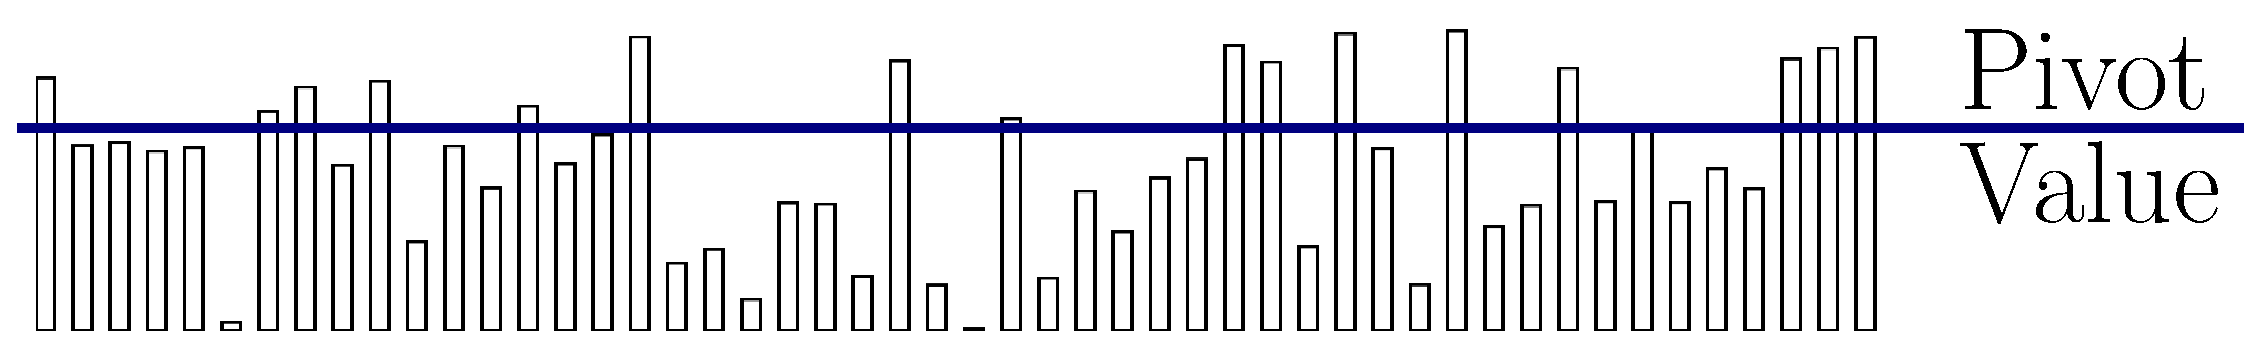
\includegraphics[width=\linewidth]{imgs/partitionDefn1Ann.eps}\\
		\vspace{1.5cm}
	}
	\onslide<2->{
		An array partitioned relative to a pivot value:\\
		\vspace{0.25cm}
		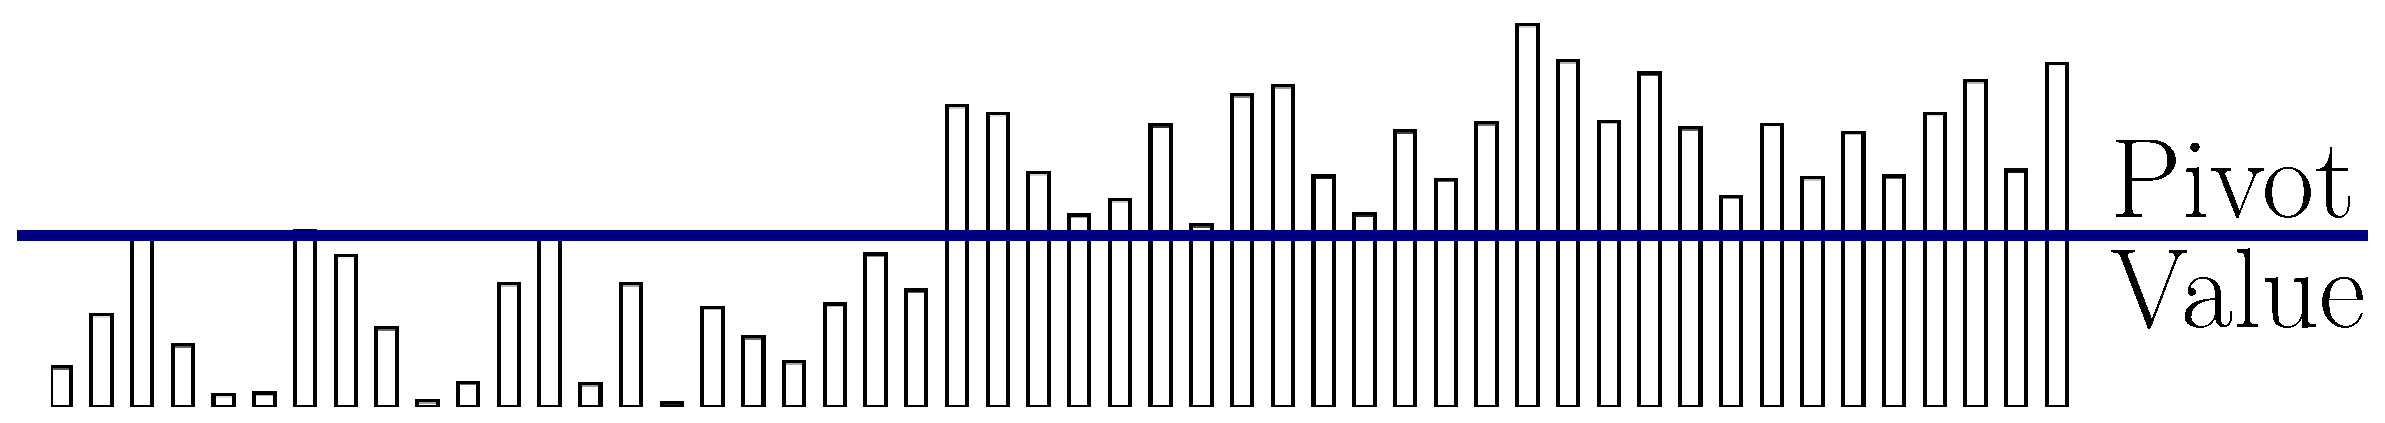
\includegraphics[width=\linewidth]{imgs/partitionDefn2Ann.eps}
	}
\end{frame}

% \begin{frame}[t]{The Partition Problem}
%   \begin{center}
%     \begin{figure}
%       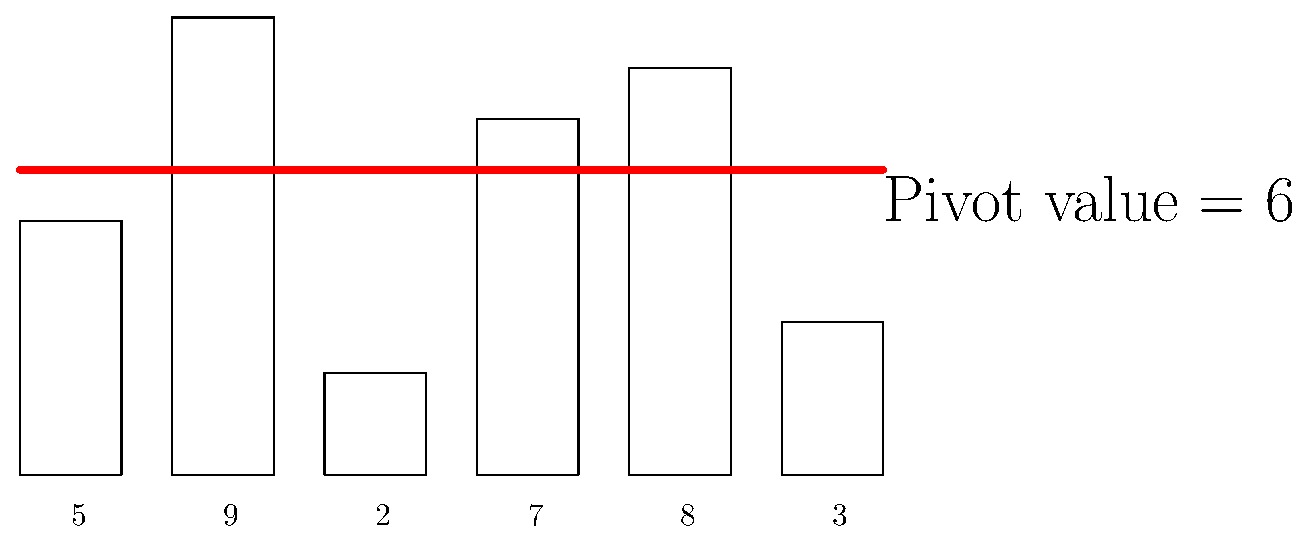
\includegraphics[width=\linewidth]{imgs/partitionDefinitionExplanation.eps}
%     \end{figure}
%   \end{center}
% \end{frame}

% \begin{frame}[t]{The Partition Problem}
%   \begin{center}
%     \begin{figure}
%       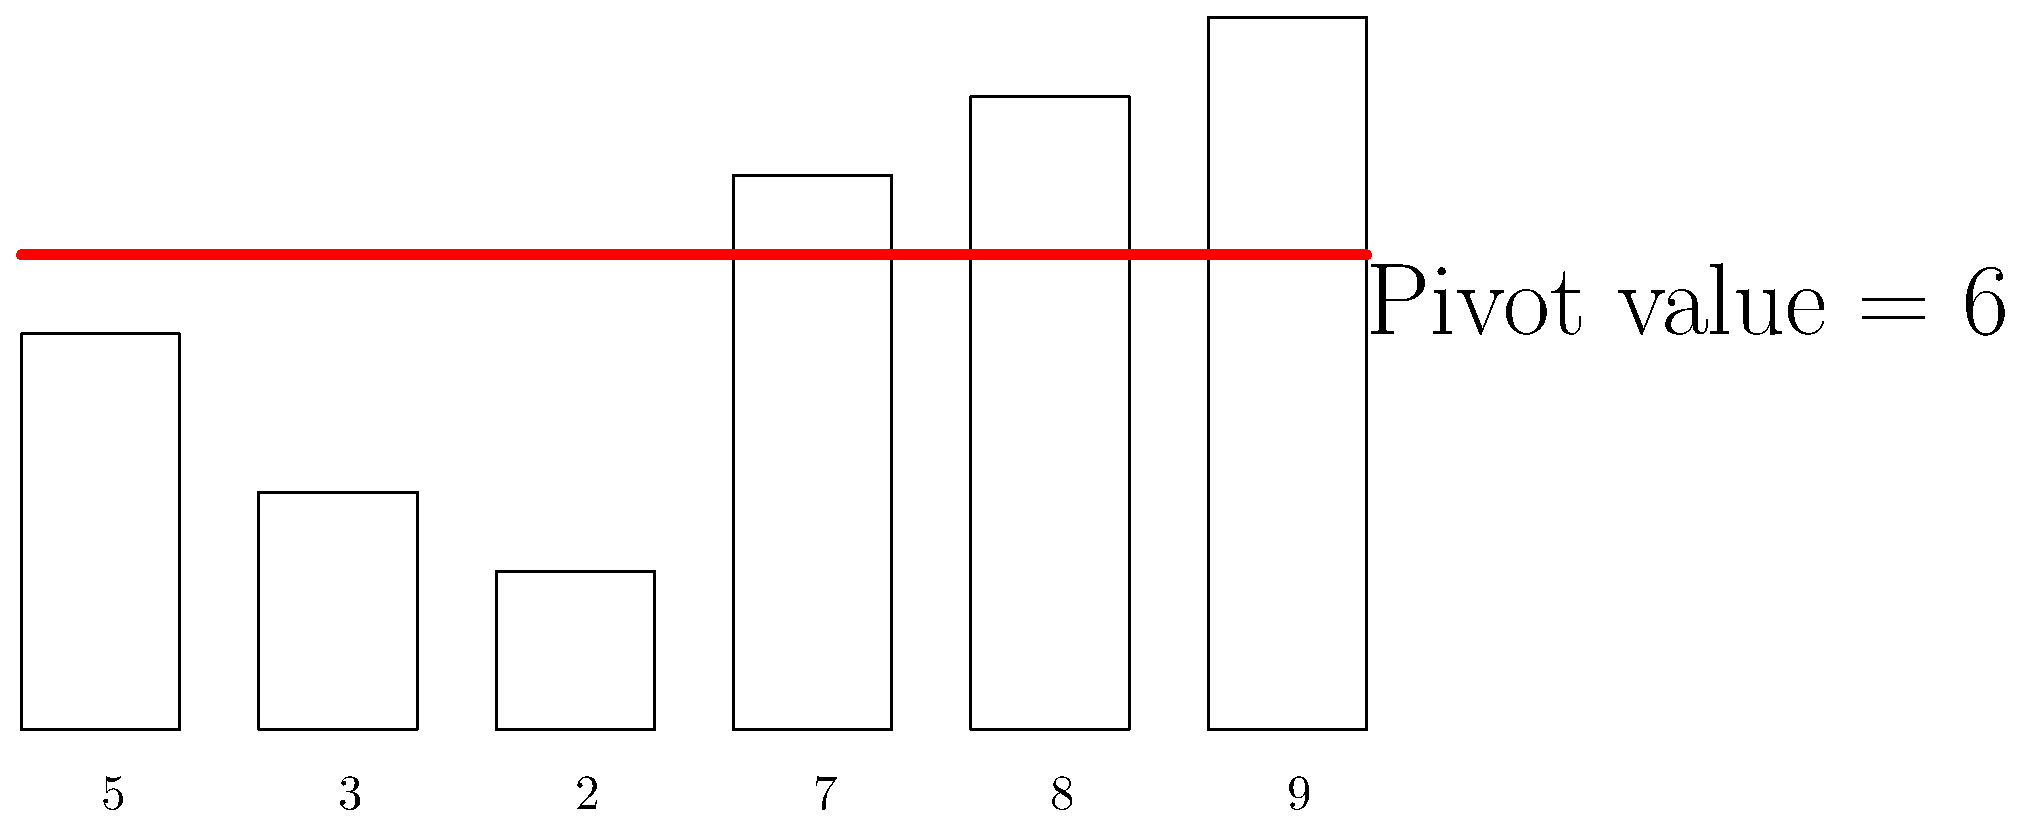
\includegraphics[width=\linewidth]{imgs/partitionDefinitionExplanation2.eps}
%     \end{figure}
%   \end{center}
% \end{frame}

\begin{frame}[t]{What is a Parallel Algorithm?}

	\begin{columns}[T] % align columns
	\begin{column}{.45\textwidth}
	Fundamental primitive: \defn{Parallel for loop}
	\vspace{2cm}

        \textbf{Parallel-For $i$ from $1$ to $4$: } \\
        \hspace{1 cm} \textbf{Do }$X_i$

%	\begin{algorithmic}
%		\State \textbf{parallel-for} $i \in \{1,2,3,4\}$
%		\State \hskip0.7cm do $X_i$
%		\State \textbf{endparallel-for}
%\end{algorithmic}

	\end{column}
	\hfill
	\begin{column}{.60\textwidth}
	\begin{figure}
		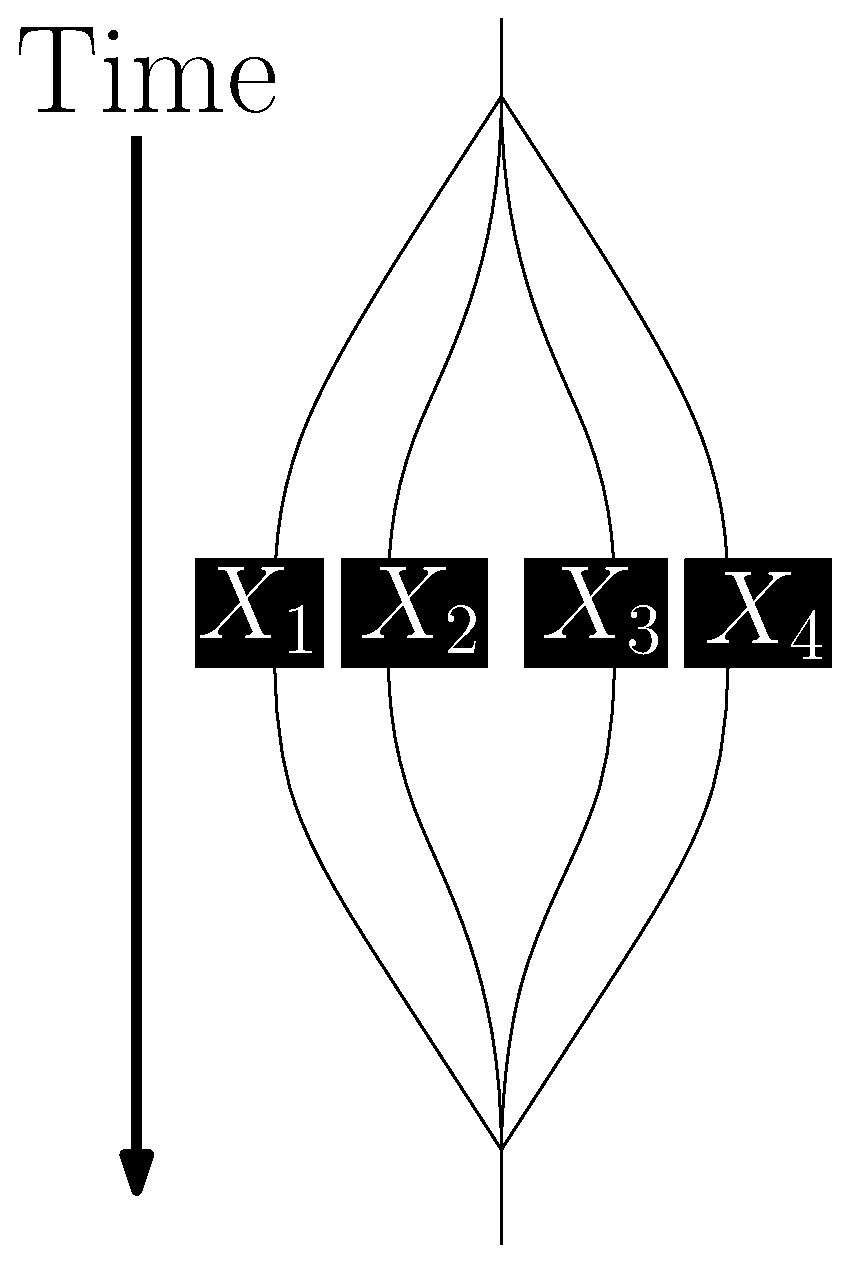
\includegraphics[width=0.75\linewidth]{imgs/altParallelForLoop.eps}
	\end{figure}
	\end{column}
	\end{columns}

\end{frame}


\begin{frame}[t]{What is a Parallel Algorithm?}
	More complicated parallel structures can be made by combining parallel for loops and recursion.
	\begin{columns}[T] % align columns
	\begin{column}{.45\textwidth}
	\end{column}
	\hfill
	\begin{column}{.60\textwidth}
		\begin{figure}
			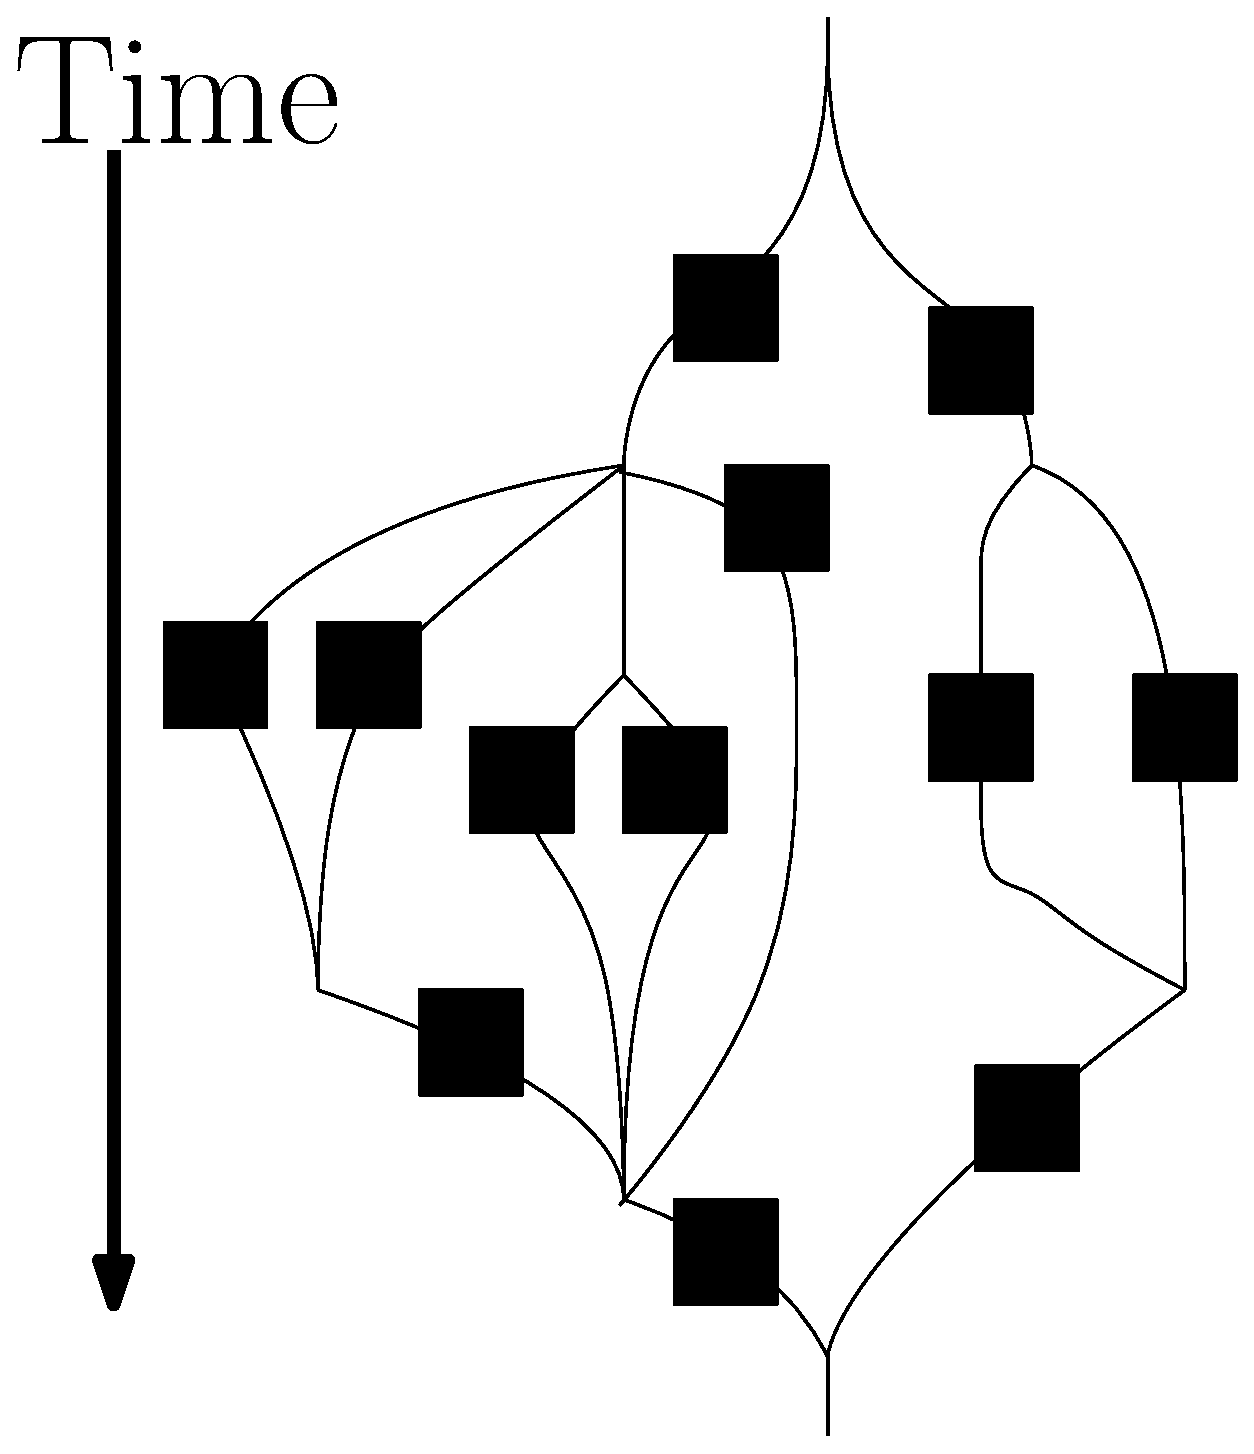
\includegraphics[width=0.8\linewidth]{imgs/altParallelForLoopComposition.eps}
		\end{figure}
	\end{column}
	\end{columns}
\end{frame}

\begin{frame}[t]{\defn{$T_p$}: Time to run on $p$ processors}
	\begin{columns}[T] % align columns
	\begin{column}{.60\textwidth}
		\begin{figure}
			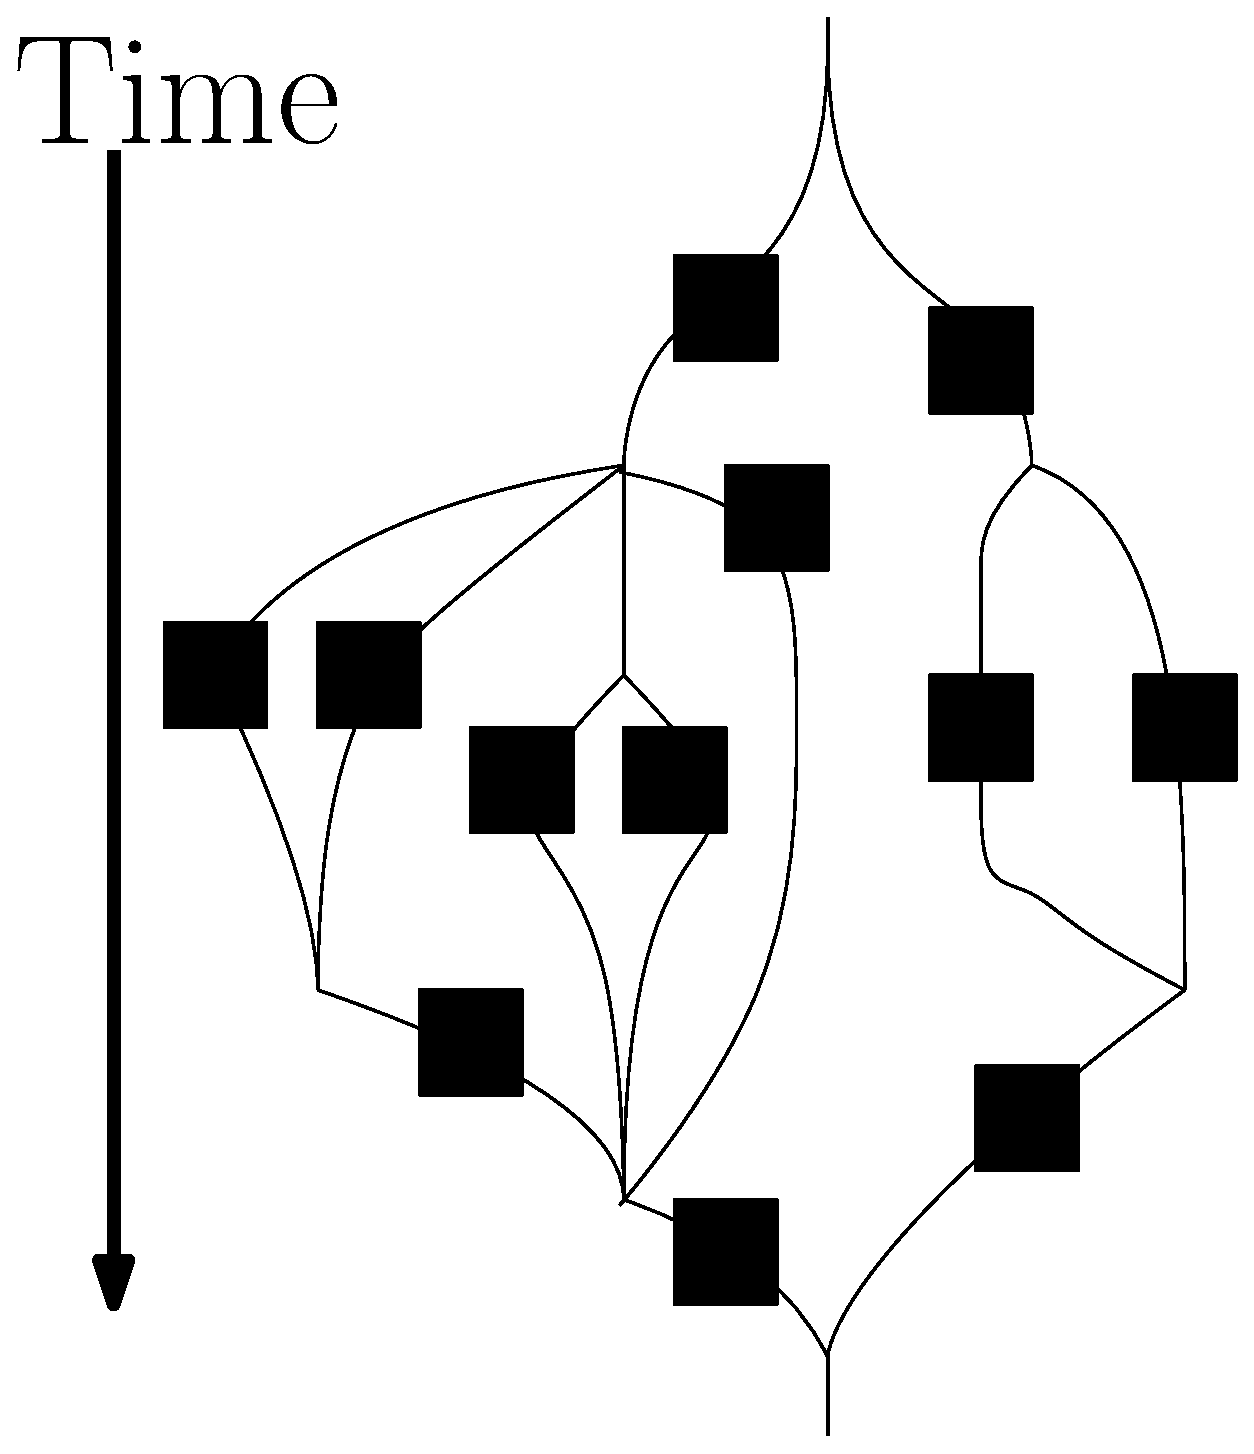
\includegraphics[width=0.8\linewidth]{imgs/altParallelForLoopComposition.eps}
		\end{figure}
	\end{column}
	\hfill
	\begin{column}{.45\textwidth}
		Important extreme cases:\\
		\vspace{0.3cm}
		\defn{Work:} $T_1$, 
		\begin{itemize}
			\item time to run in serial
			\item "sum of all work"
		\end{itemize}
		\vspace{0.3cm}
		\defn{Span:} $T_\infty$,
		\begin{itemize}
			\item time to run on infinitely many processors,\\ 
			\item "height of the graph"
		\end{itemize}	
	\end{column}
	\end{columns}
\end{frame}



\begin{frame}[t]{Bounding $T_p$ with Work and Span}
% \begin{defin}[$T_p$]
%   Running time on $p$ processors. Note: $T_p \ge T_\infty, T_p \ge \frac{T_1}{p}$.
% \end{defin}	
% \begin{defin}[Work]
%   Running time on a single processor. $T_1 = \sum_i W_i$.
% \end{defin}	
% \begin{defin}[Span]
%   Running time on infinitely many processors. $T_\infty = \sum_i 1$.
% \end{defin}	
	\defn{Brent's Theorem:} \citefont{[Brent, 74]}
% \begin{theorem}[Brent's Theorem]
	% $$T_p = \sum_i \Big\lceil \frac{W_i}{p} \Big\rceil \le \sum_i \Big( \frac{W_i}{p}+1 \Big) = \frac{T_1}{p}+T_\infty.$$	
	$$T_p = \Theta\left(\frac{T_1}{p}+T_\infty\right)$$
% \end{theorem}
	$ $\\ \vspace{1cm}
	\textbf{Take away:} Work $T_1$ and span $T_\infty$ determine $T_p$.
\end{frame}


\begin{frame}[t]{The Standard Parallel Partition Algorithm}
\begin{table}[]
\begin{tabular}{ll}
	\emph{Step}                                              & \emph{Span} \\\\
Create filtered array                             & $O(1)$            \\\\
Compute prefix sums of filtered array & $O(\log n)$       \\\\
Use prefix sums to partition array                & $O(1)$           
\end{tabular}
\end{table}
\vspace{10 mm}
Total span: $O(\log n)$
\end{frame}

\begin{frame}[t]{The Problem}
	\onslide<1->{Why is the Standard Algorithm is slow in practice?}
	\begin{columns}[T] % align columns
	\begin{column}{.65\textwidth}
	\begin{itemize}
		\item<2-> Uses extra memory % not in place
		\item<3-> Makes multiple passes over array
	\end{itemize}
	\end{column}
	\begin{column}{.35\textwidth}
	\onslide<4->{\hspace{-1cm}$\Biggr\}\text{ "bad cache behavior"}$}
	\end{column}
	\end{columns}
	\vspace{0.4 cm}

	\onslide<5->{But fastest algorithms in practice lack theoretical guarantees}
	\begin{itemize}
		\item<6-> Lock-based and atomic-variable based algorithms
		\item<7-> The Strided Algorithm\\ \citefont{[Francis and Pannan, 92; Frias and Petit, 08]}\\ 
		\onslide<8->{No locks or atomic-variables,\\but no bound on span in general}
	\end{itemize}
	\onslide<9-> {
	\vspace{0.4cm}
	\textbf{Our Question:}
Can we create an algorithm with theoretical guarantees that is fast in practice?}
\end{frame}

% \begin{frame}[t]{Cache Efficiency}
%   Rough definition:\\
%   The number of passes over the input data. \\
%   \vspace{1cm}
%   A cache-efficient algorithm will make relatively few requests to load data from memory into cache where it can be manipulated. \\
%   \vspace{1cm}
%   Poor cache behavior will harm an algorithms performance in practice.
% \end{frame}

\begin{frame}[t]{Our Result}
	We created a randomized algorithm for the parallel partition problem: the \defn{Smoothed-Striding Algorithm}.\\
	\vspace{0.5cm}
	The Smoothed-Striding algorithm has...
	\begin{itemize}
		\item performance comparable to that of the Strided Algorithm
		\item polylogarithmic span like the Standard Algorithm
		\item theoretically optimal cache behavior 
	\end{itemize}
\end{frame}

% \begin{frame}[t]{The Smoothed-Striding Algorithm's performance}
%   \begin{figure}
%     \begin{center}
%       \CILKtable
%     \end{center}
%   \end{figure}
% \end{frame}

\begin{frame}[t]{Algorithm Comparison}
	\begin{columns}[T] % align columns
	\begin{column}{.45\textwidth}
		\textbf{Strided Algorithm}\\\citefont{[Francis and Pannan, 92; Frias and Petit, 08]}\\
		\vspace{0.25cm}
		\begin{itemize}
			\item Good cache behavior in practice\\\hfill
			\item Worst case span is $T_\infty \approx n$\\\hfill
			\item But: on random inputs span is $T_\infty = \tilde{O}(n^{2/3})$
		\end{itemize}
	\end{column}
	\hfill
	\begin{column}{.55\textwidth}
		\textbf{Smoothed-Striding Algorithm}\\\citefont{}\\
		\vspace{0.25cm}
		\begin{itemize}
			\item Provably optimal cache behavior\\\hfill
			\item Span is $O(\log n \log\log n)$ with high probability in $n$\\\hfill
			\item Uses randomization inside the algorithm to remove the need for randomized input
		\end{itemize}
	\end{column}
	\end{columns}
\end{frame}

\begin{frame}[t]{Speedup over Serial Partition: Smoothed-Striding Algorithm's performance}
	\begin{figure}
		\begin{center}
			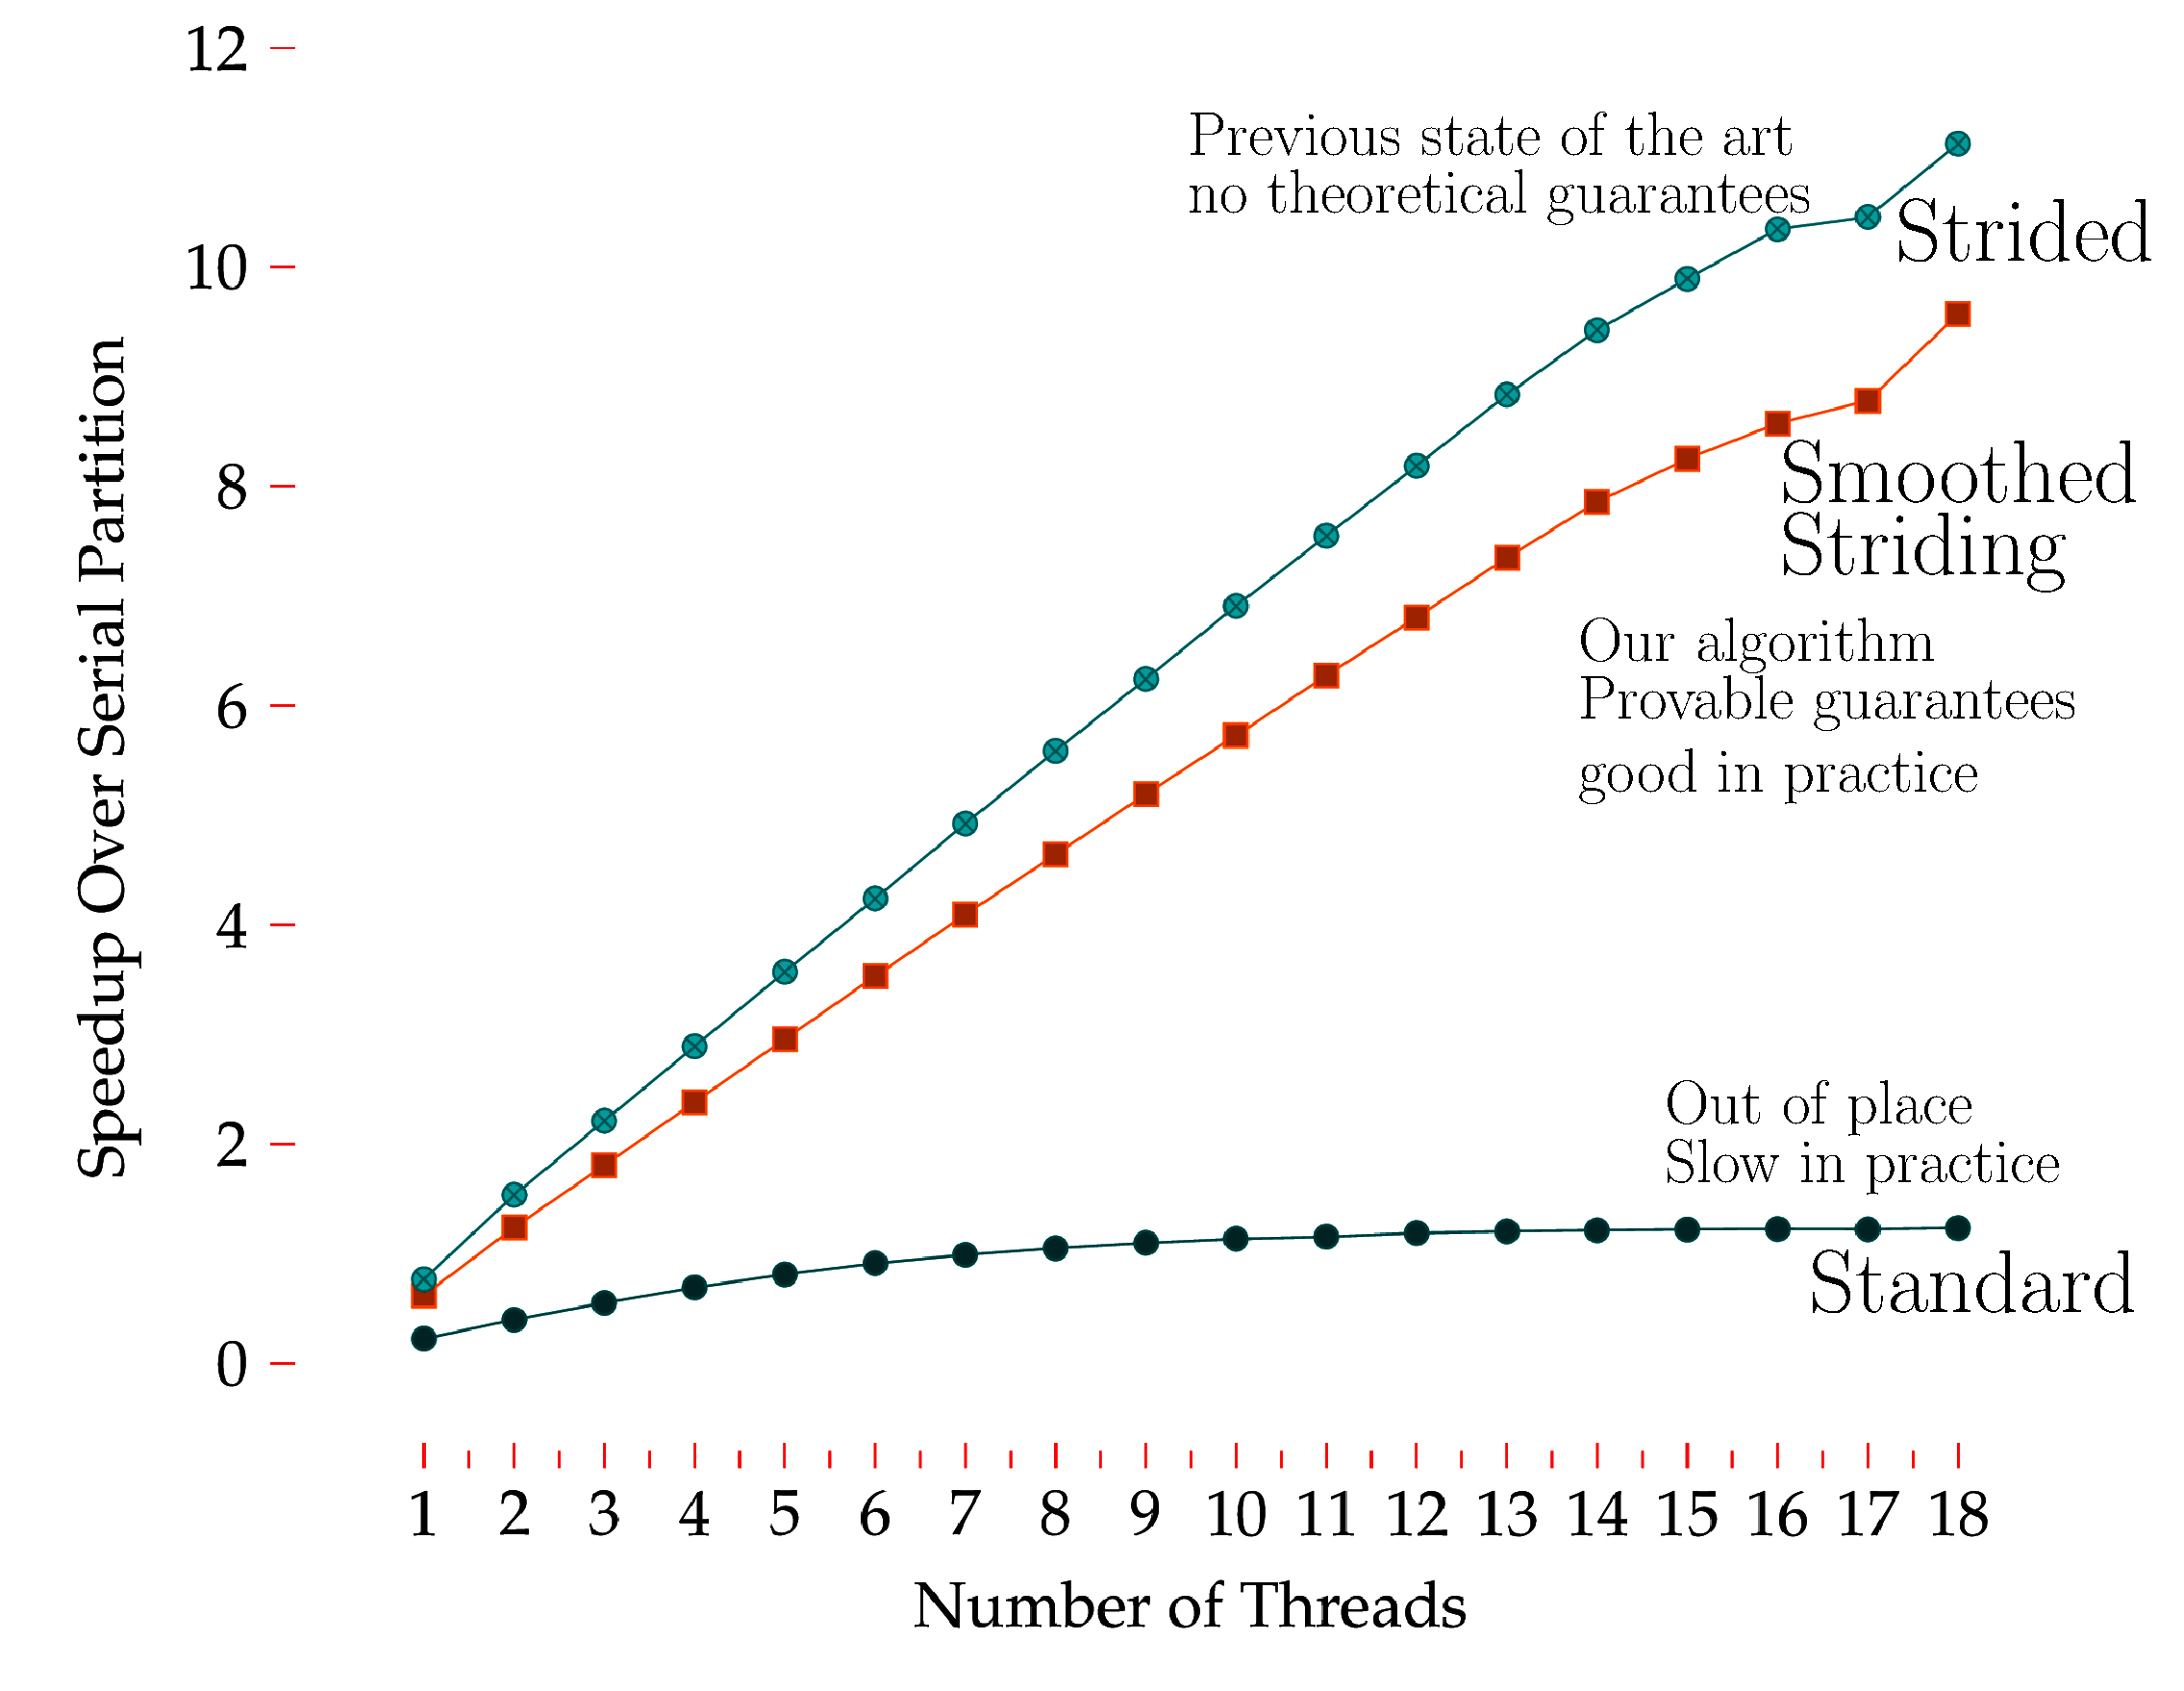
\includegraphics[width=0.9\linewidth]{imgs/compiledGraph.eps}
		\end{center}
	\end{figure}
\end{frame}

% \begin{frame}[t]{Randomized Algorithms}
%   \defn{With high probability in $n$:}
%     $$1-\frac{1}{n^c}$$
%   Can be made arbitrarily close to $1$ by choice of $c$.
% \end{frame}

% \begin{frame}[t]{Memory Bandwidth Bound}
%   \begin{defin}[Cache miss]
%     A cache miss occurs when the algorithm must load a cache-line not stored in cache into cache.
%   \end{defin}	
%   \begin{itemize}
%     \item In-place $\implies$ spatial-locality  
%     \item Kuszmaul developed in-place parallel partition algorithm
%       \begin{itemize}
%         \item Outperforms standard out-of-place algorithm
%         \item Outperformed by more cache-efficient higher span algorithm
%       \end{itemize}
%     \item Experiments show Memory Bandwidth Bound (incurring too many cache misses) is the problem
%     \item Want Temporal and Spatial locality
%   \end{itemize}
% \end{frame}


% \begin{frame}[t]{The Serial Partition Algorithm}
% \begin{figure}
%     \begin{overprint}
%       \onslide<1>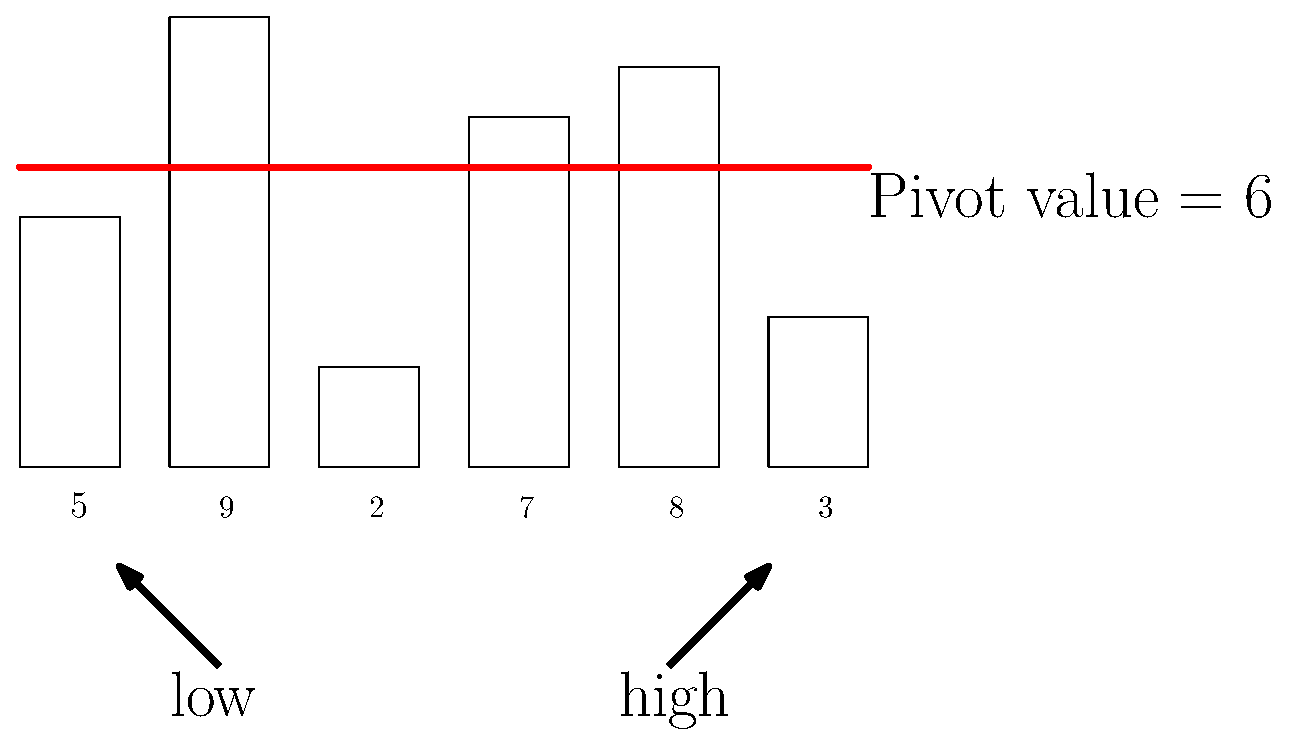
\includegraphics[width=\linewidth]{imgs/serialPartition1.eps}
%     \onslide<2>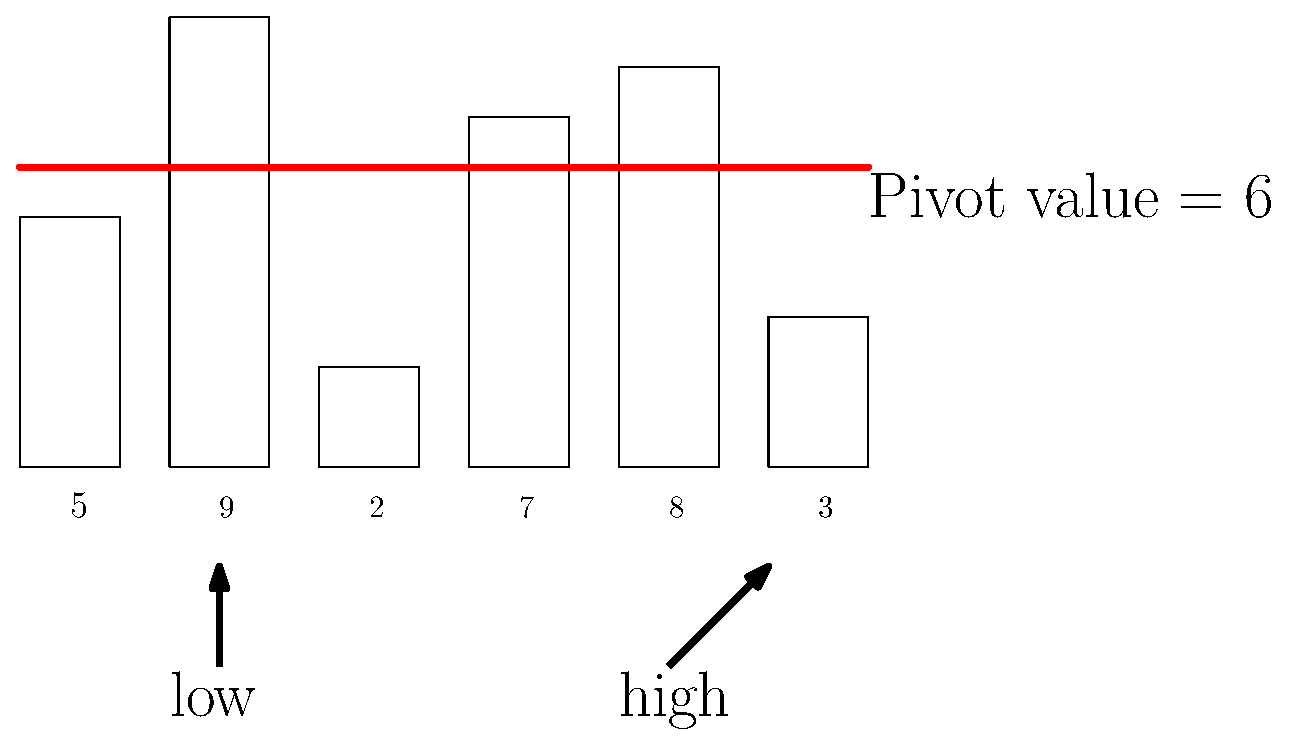
\includegraphics[width=\linewidth]{imgs/serialPartition2.eps}
%     \onslide<3>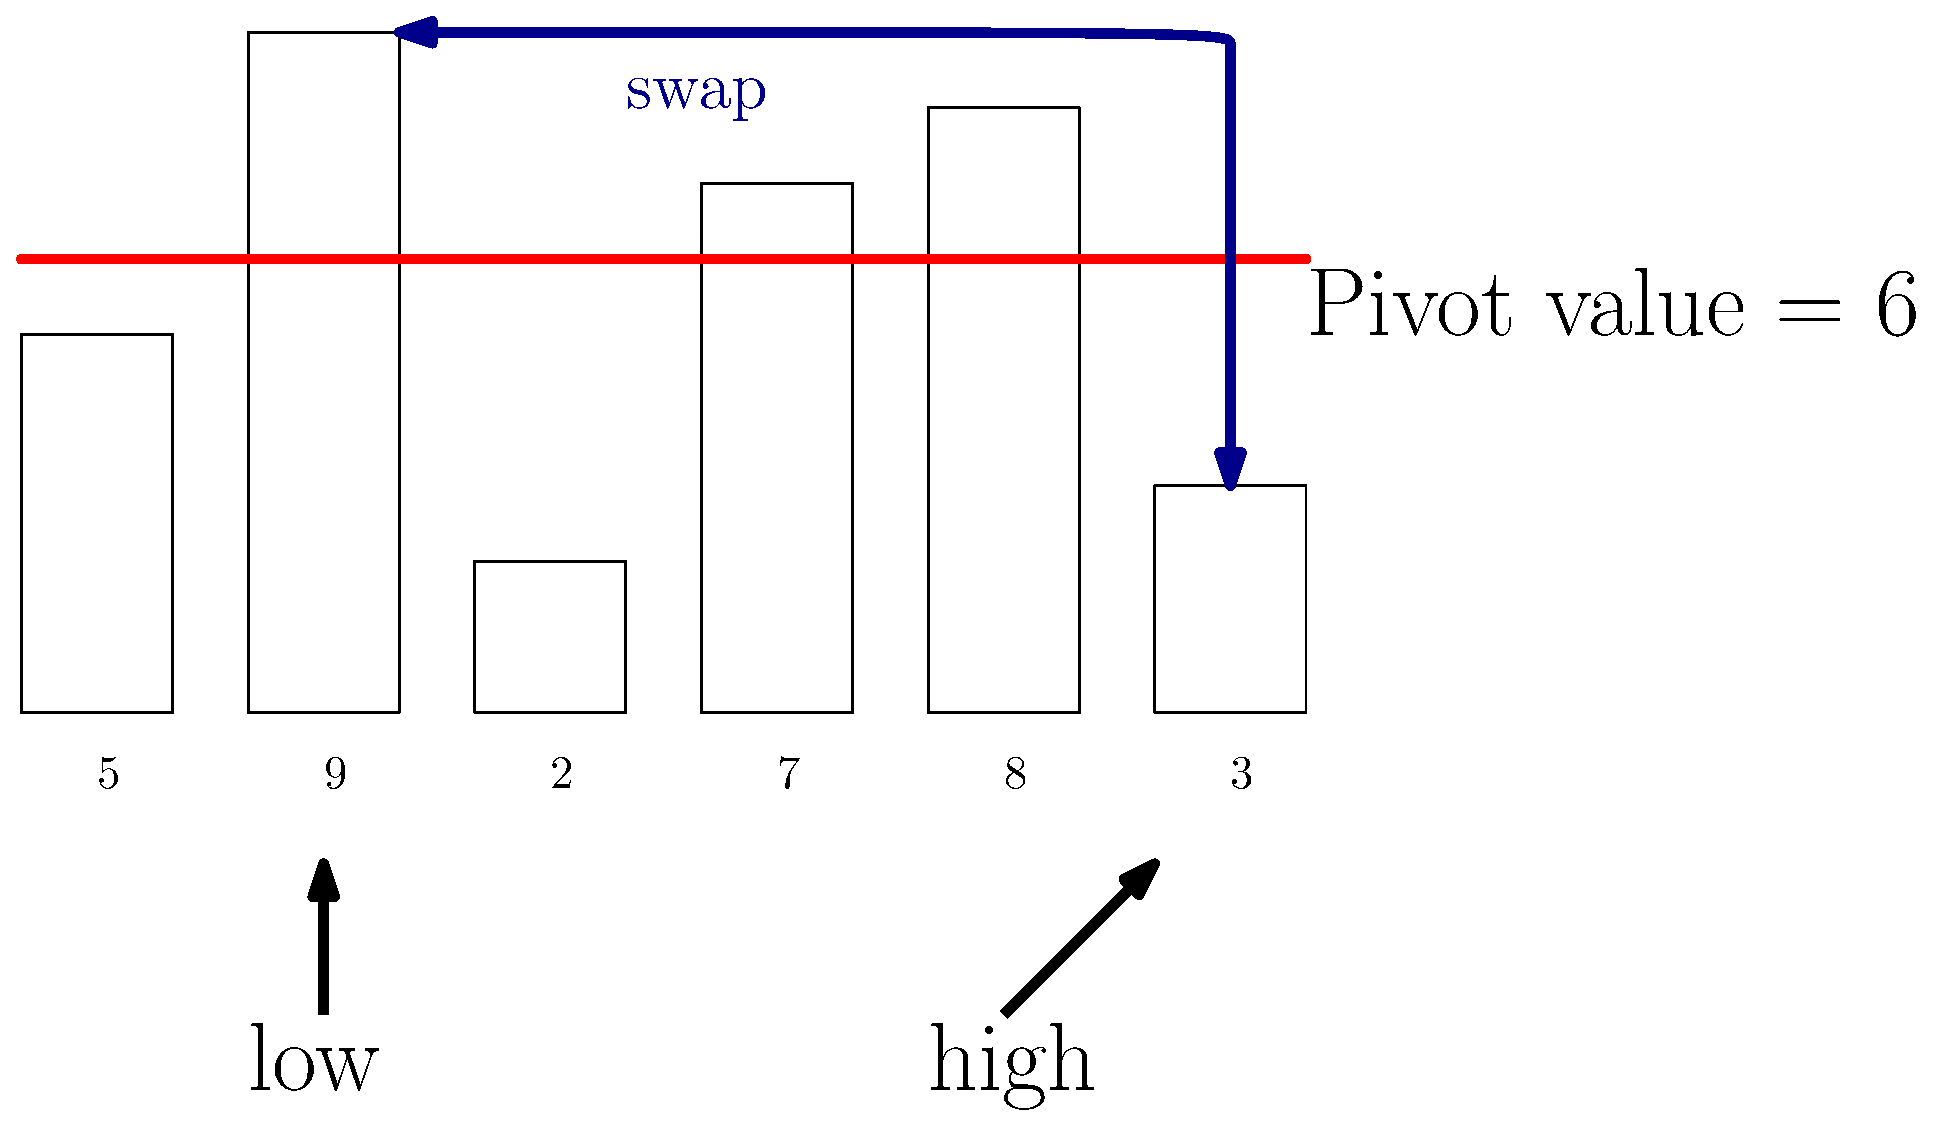
\includegraphics[width=\linewidth]{imgs/serialPartition3.eps}
%     \onslide<4->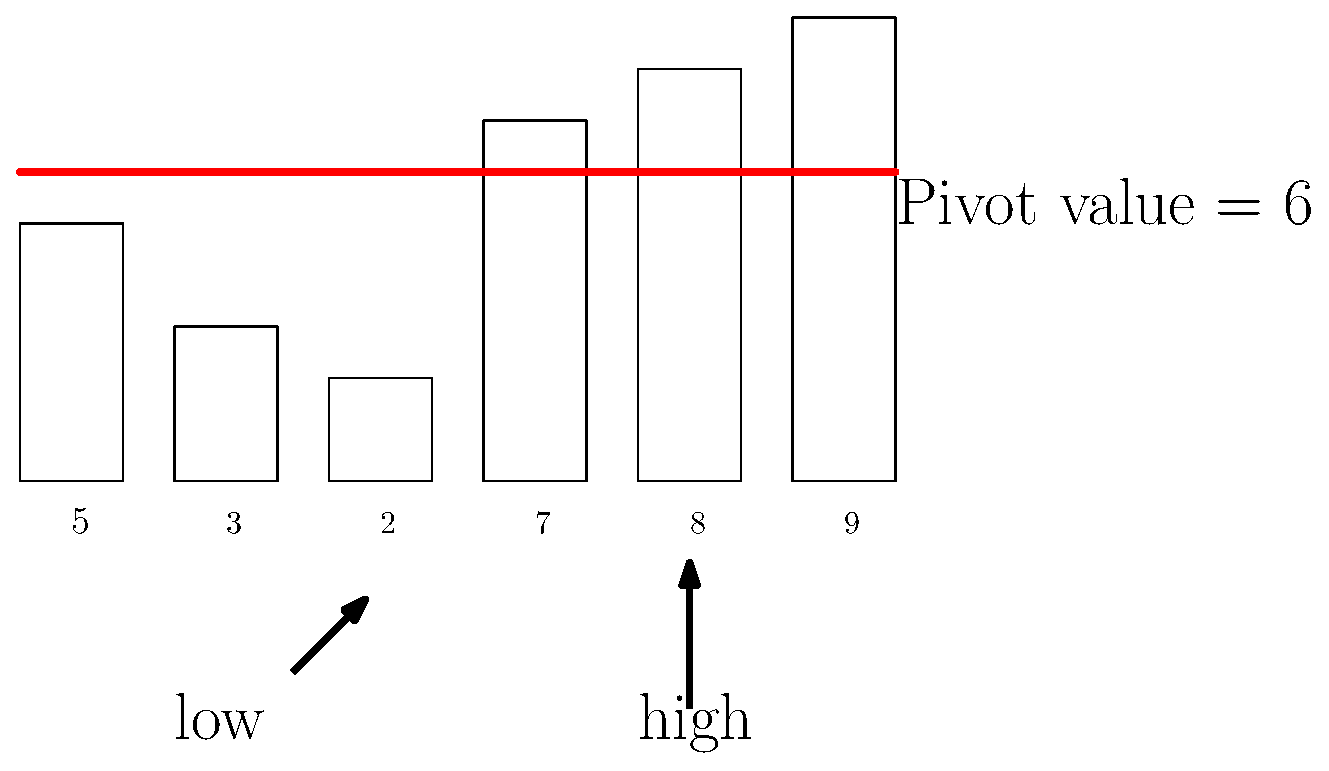
\includegraphics[width=\linewidth]{imgs/serialPartition4.eps}
%     \end{overprint}
%   \end{figure}	
% \end{frame}

\begin{frame}[t]{}
	\vfill
	\begin{center}
		{\Huge The Strided Algorithm}\\
		\citefont{[Francis and Pannan, 92; Frias and Petit, 08]}
	\end{center}
	\vfill
\end{frame}


%% BILL NOTES:
%% extra slide introducing v_i (v_4?...)
%% extra slide for partition vmin through vmax in serial 

\begin{frame}[t]{}%{Strided Algorithm Description}
	\vspace{0.25cm}
	\begin{overprint}
	\onslide<1>Logically partition the array into chunks of adjacent elements:
	\onslide<2>Form groups $P_i$ where $P_i$ contains the $i$-th element from each chunk:
	\onslide<3>Perform serial partitions on each $P_i$ in parallel over the $P_i$'s:
	\onslide<4>Identify the splitting index $v_i$ (the first element greater than the pivot) of each $P_i$. 
	\onslide<5>Partition the subarray from the minimum splitting index to the maximum splitting index in serial. This completes the partition. 
	\end{overprint}
	\vspace{0.25cm}
	\begin{overprint}
	\onslide<1>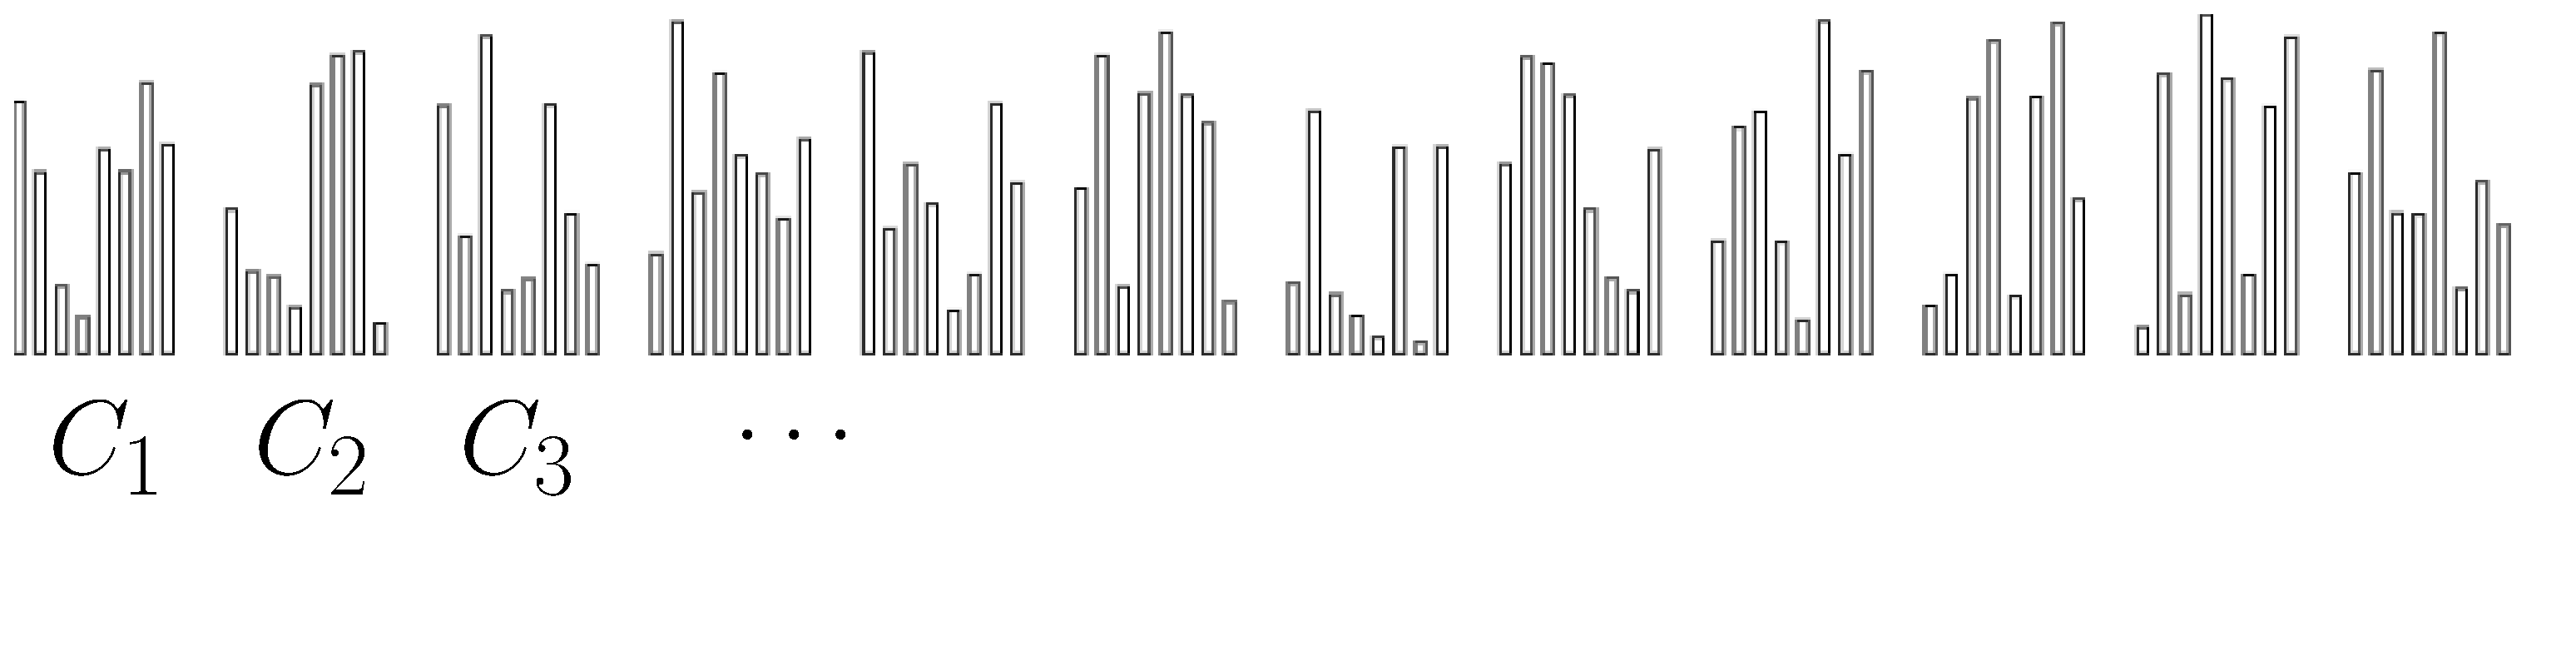
\includegraphics[width=\linewidth]{imgs/stridedAlgSim1Ann.eps}
	\onslide<2>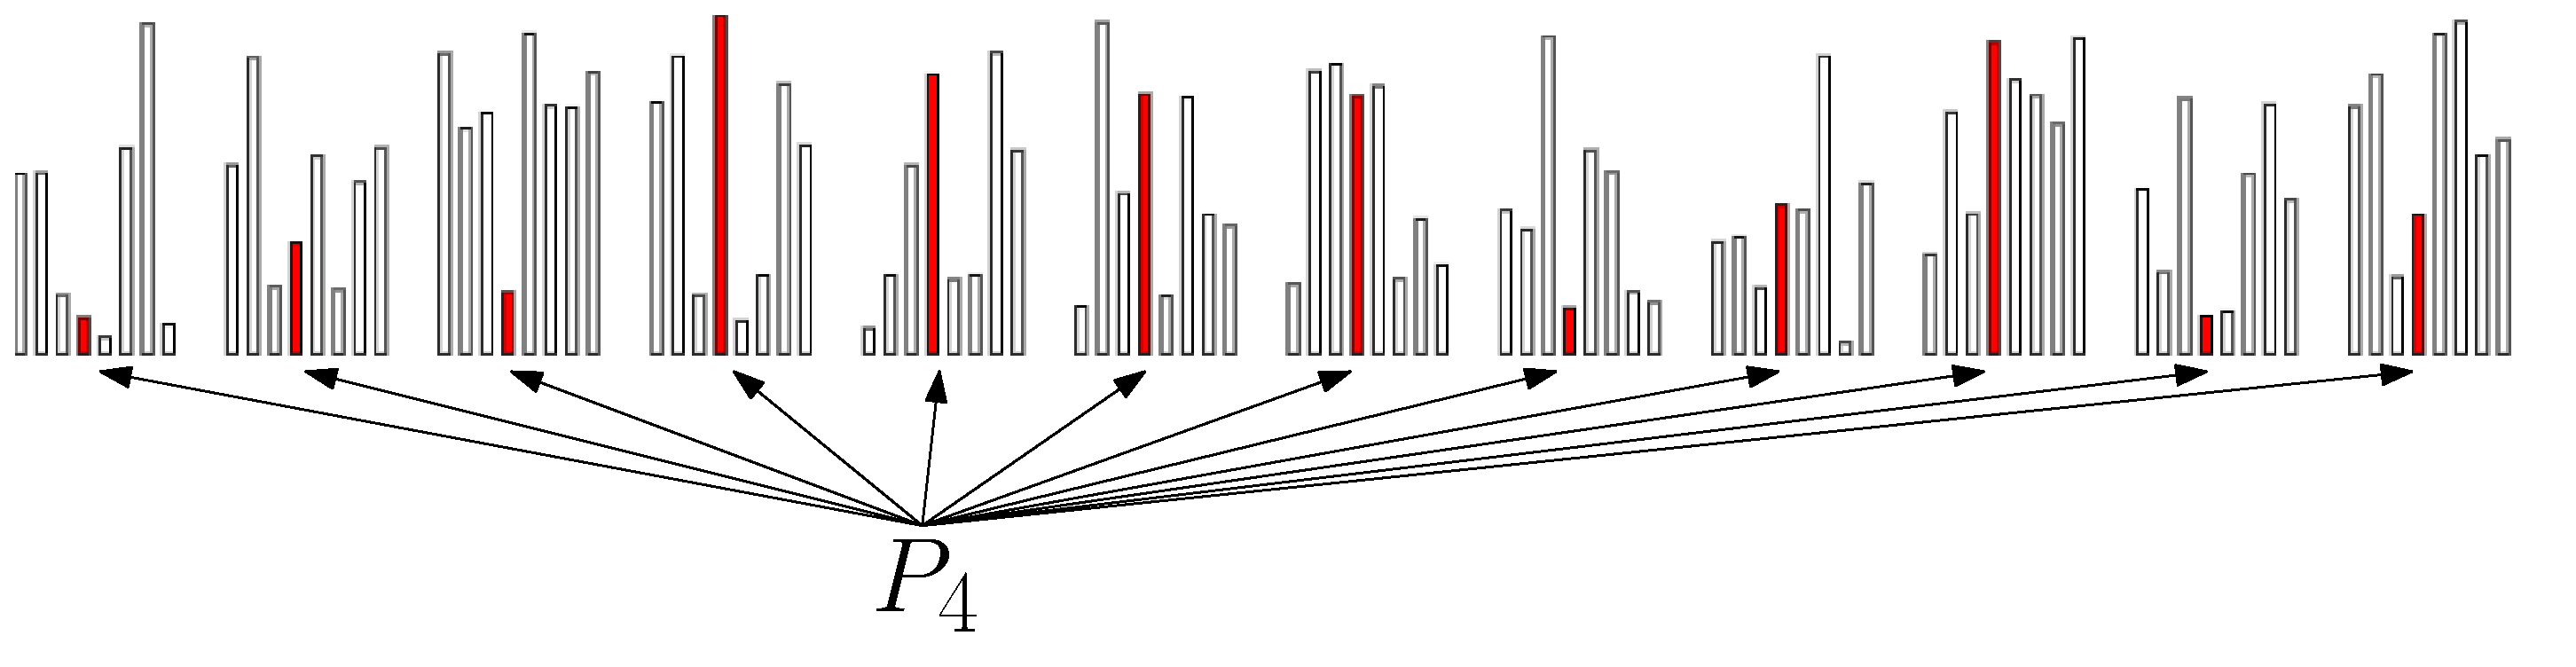
\includegraphics[width=\linewidth]{imgs/stridedAlgSim2Ann.eps}
	\onslide<3>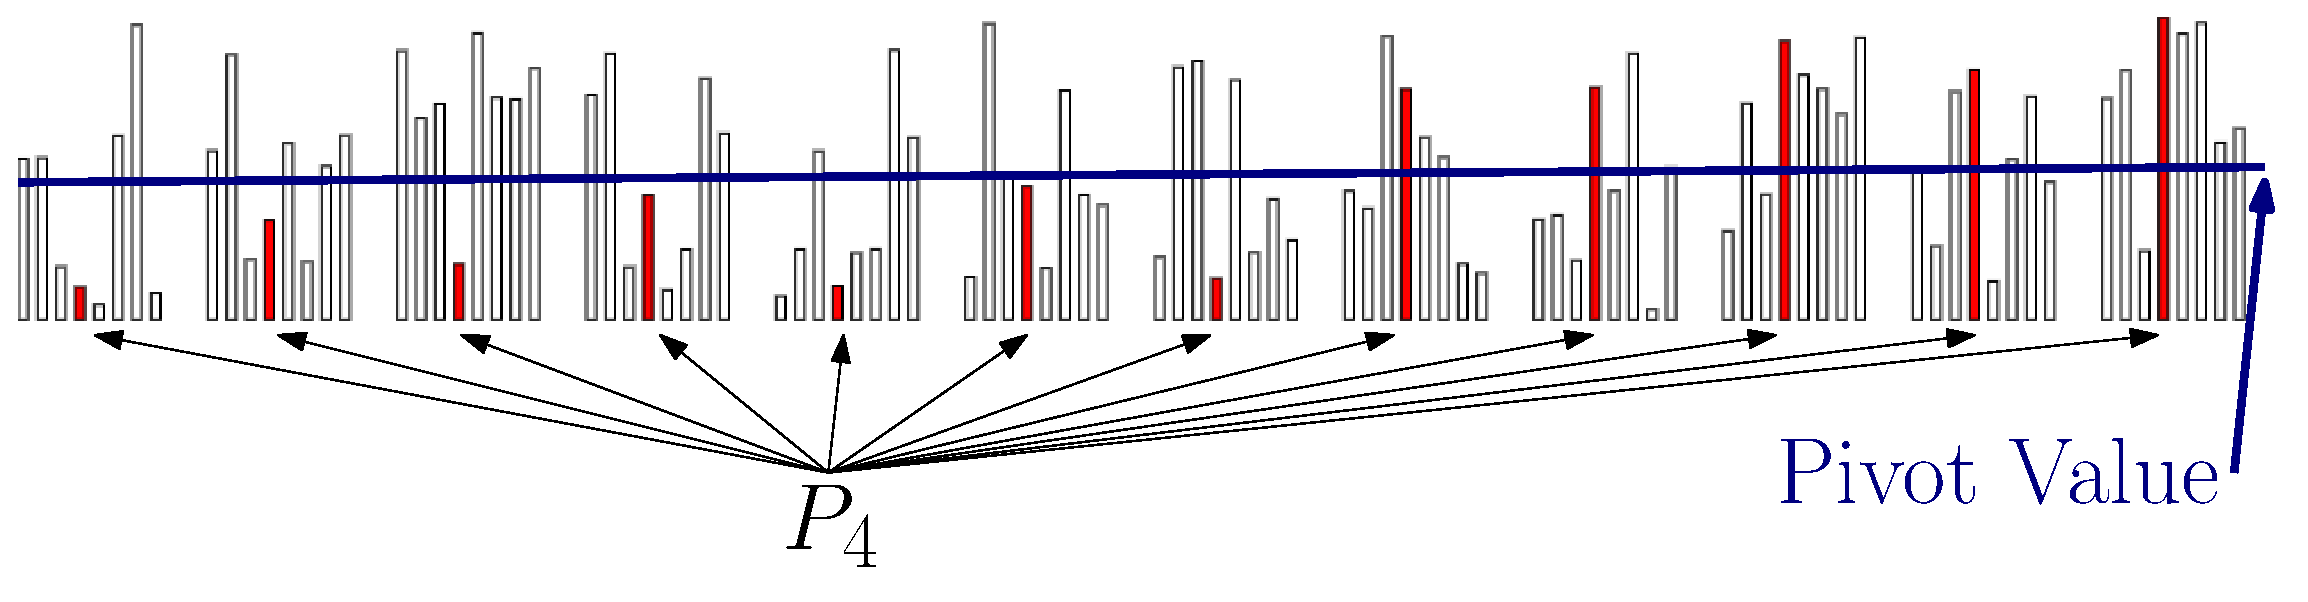
\includegraphics[width=\linewidth]{imgs/stridedAlgSim3Ann.eps}
	\onslide<4>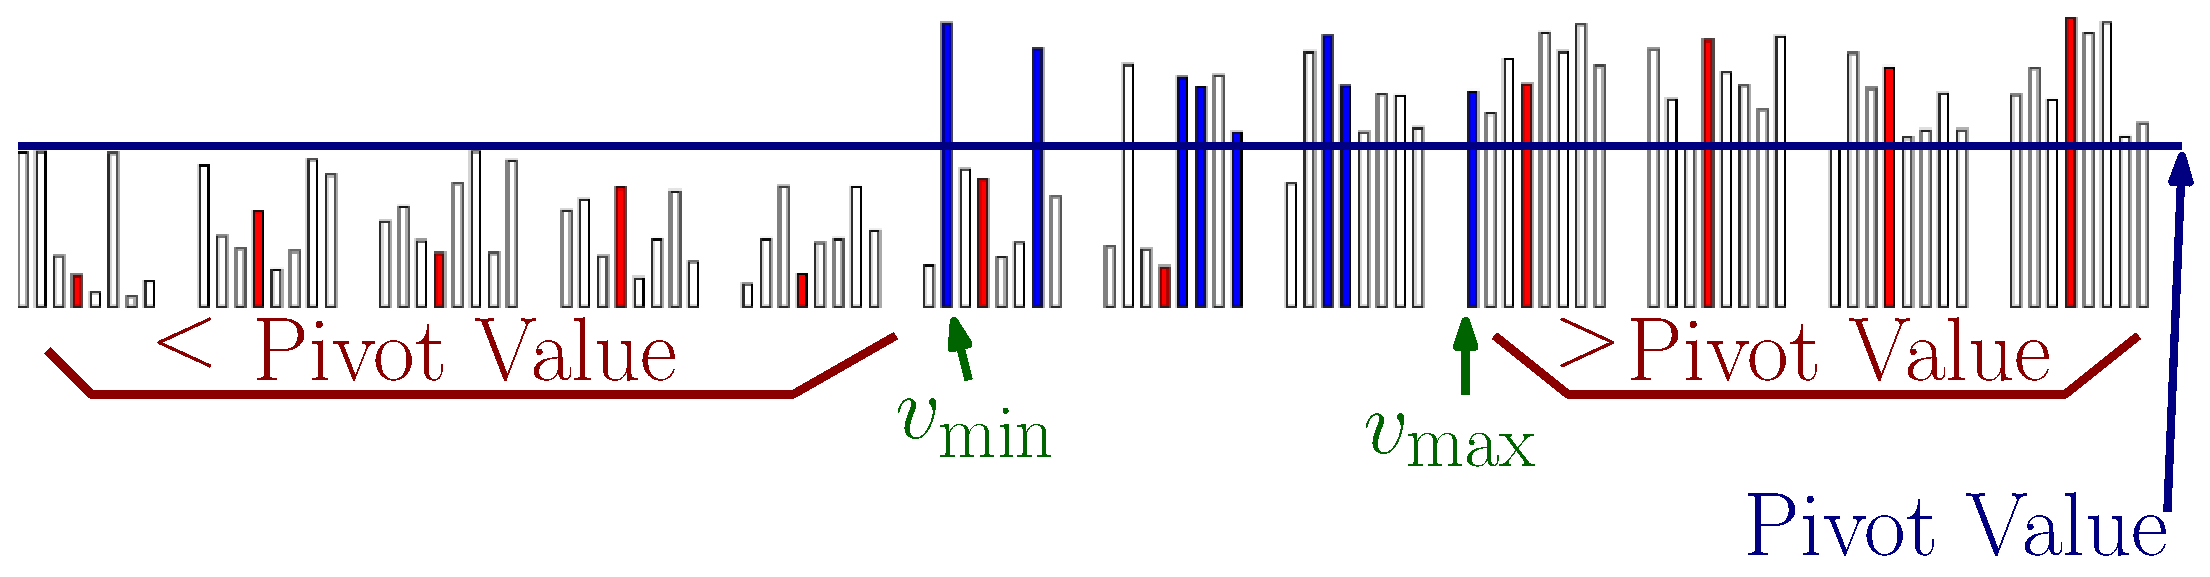
\includegraphics[width=\linewidth]{imgs/stridedAlgSim4Ann.eps}
	\onslide<5>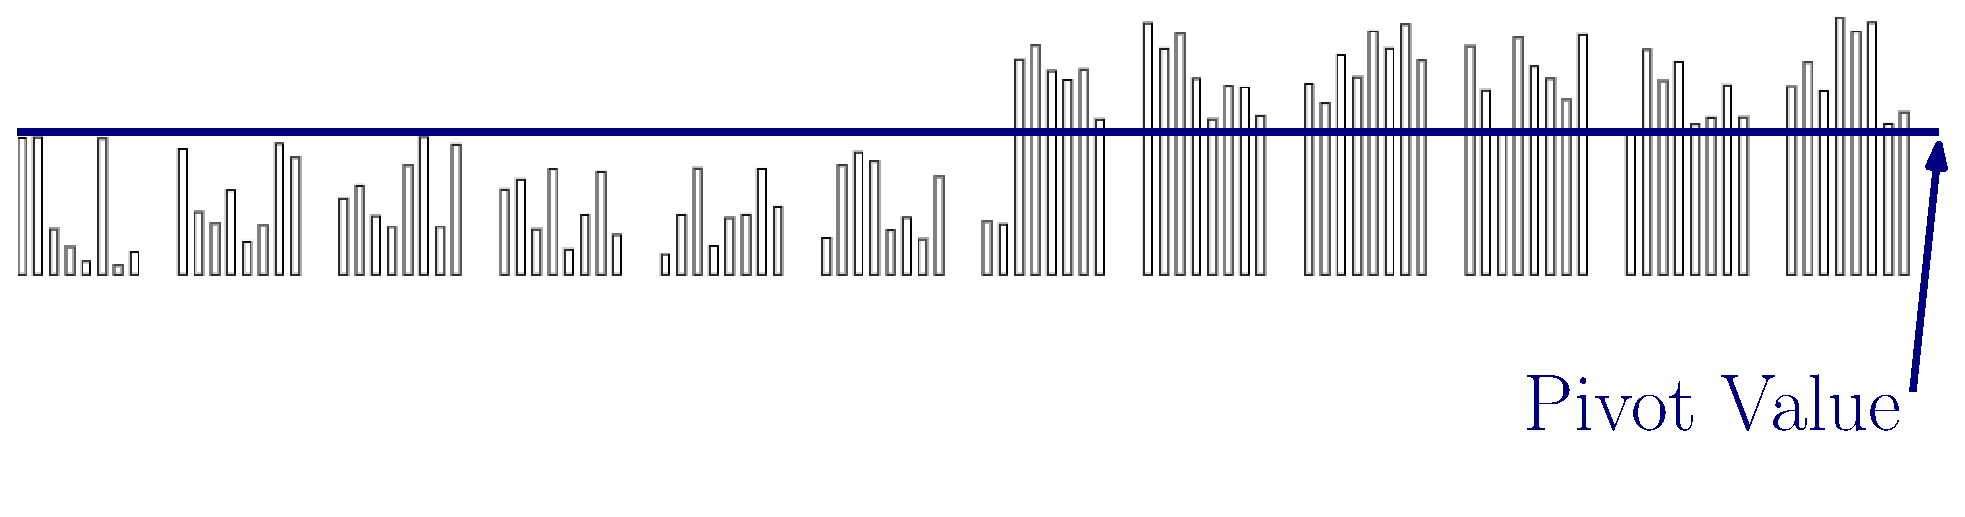
\includegraphics[width=\linewidth]{imgs/stridedAlgSim5Ann.eps}
	\end{overprint}
	\vspace{0.25cm}
	\begin{overprint}
	\onslide<3>This step is highly parallel.
	% \onslide<4>Note that all elements below the minimum splitting index are less than the pivot and all elements greater than the maximum splitting index are greater than the pivot.
	\onslide<5> Note that this step has no parallelism. In general this results in span $O(n)$. However, if the number of elements less than the pivot in each $P_i$ is similar, then size of the subarray to be partitioned can be very small.
	\end{overprint}
\end{frame}

\begin{frame}[t]{}%{Strided Algorithm Description}
	\vspace{0.25cm}
	\begin{overprint}
	\onslide<1>Logically partition the array into chunks of adjacent elements:
	\onslide<2>Form groups $P_i$ where $P_i$ contains the $i$-th element from each chunk:
	\onslide<3>Perform serial partitions on each $P_i$ in parallel over the $P_i$'s:
	\onslide<5>Identify the splitting index $v_i$ (the first element greater than the pivot) of each $P_i$. 
	\onslide<7>Partition the subarray from the minimum splitting index to the maximum splitting index in serial. This completes the partition. 
	\end{overprint}
	\vspace{0.25cm}
	\begin{overprint}
	\onslide<1>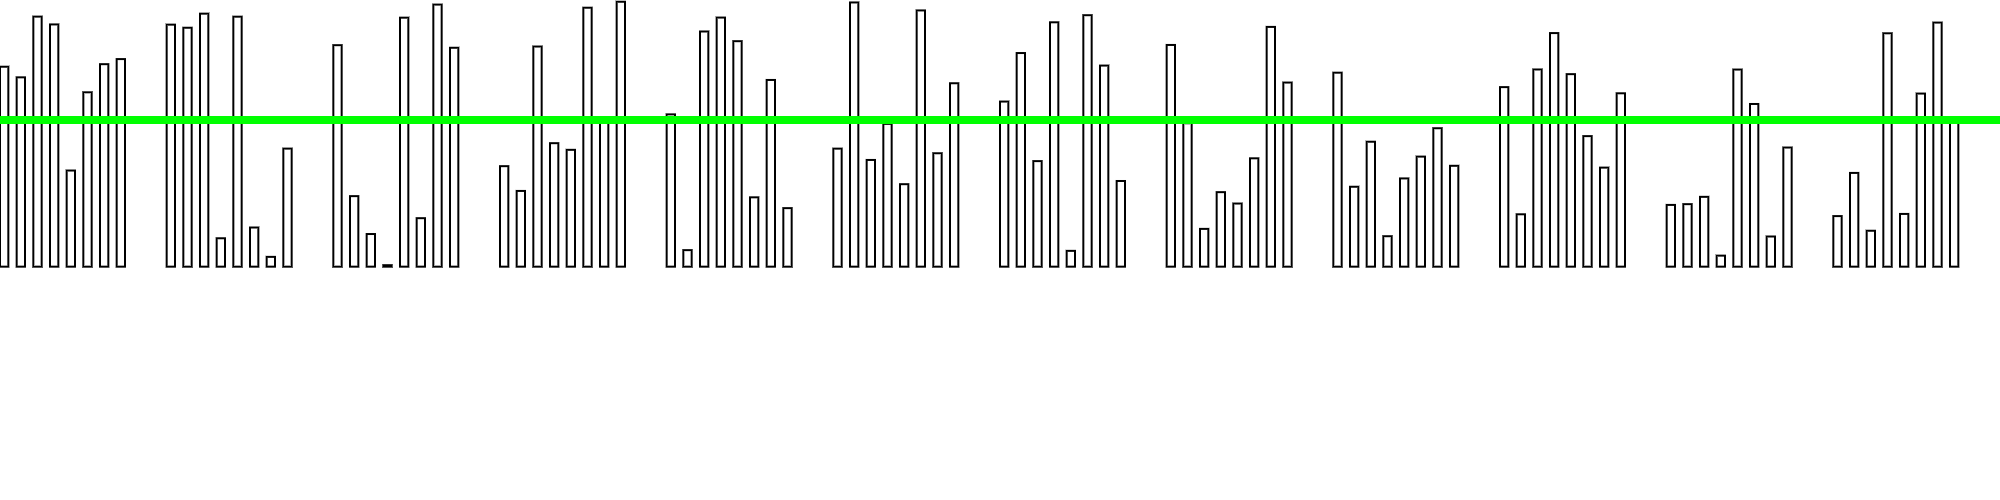
\includegraphics[width=\linewidth]{imgs/stridedAlgSim/stridedAlgSim_1.png}
	\onslide<2>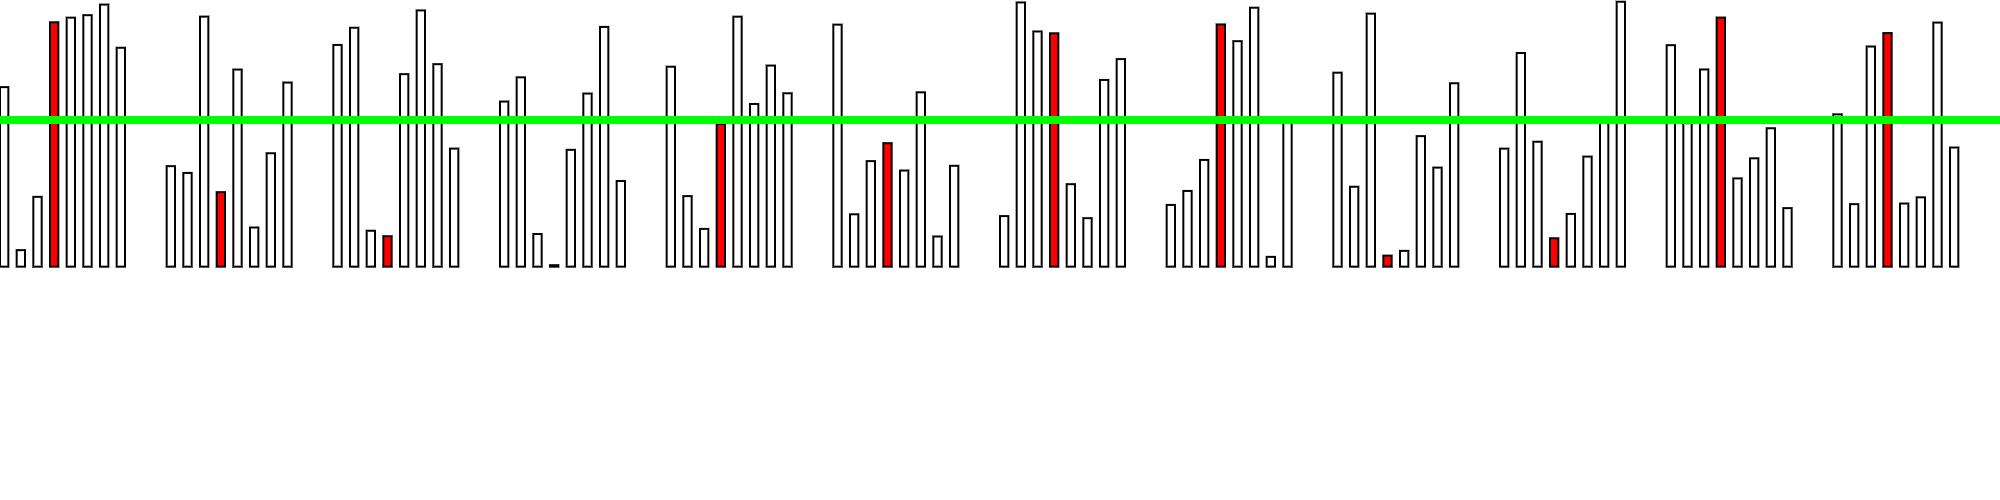
\includegraphics[width=\linewidth]{imgs/stridedAlgSim/stridedAlgSim_2.png}
	\onslide<3>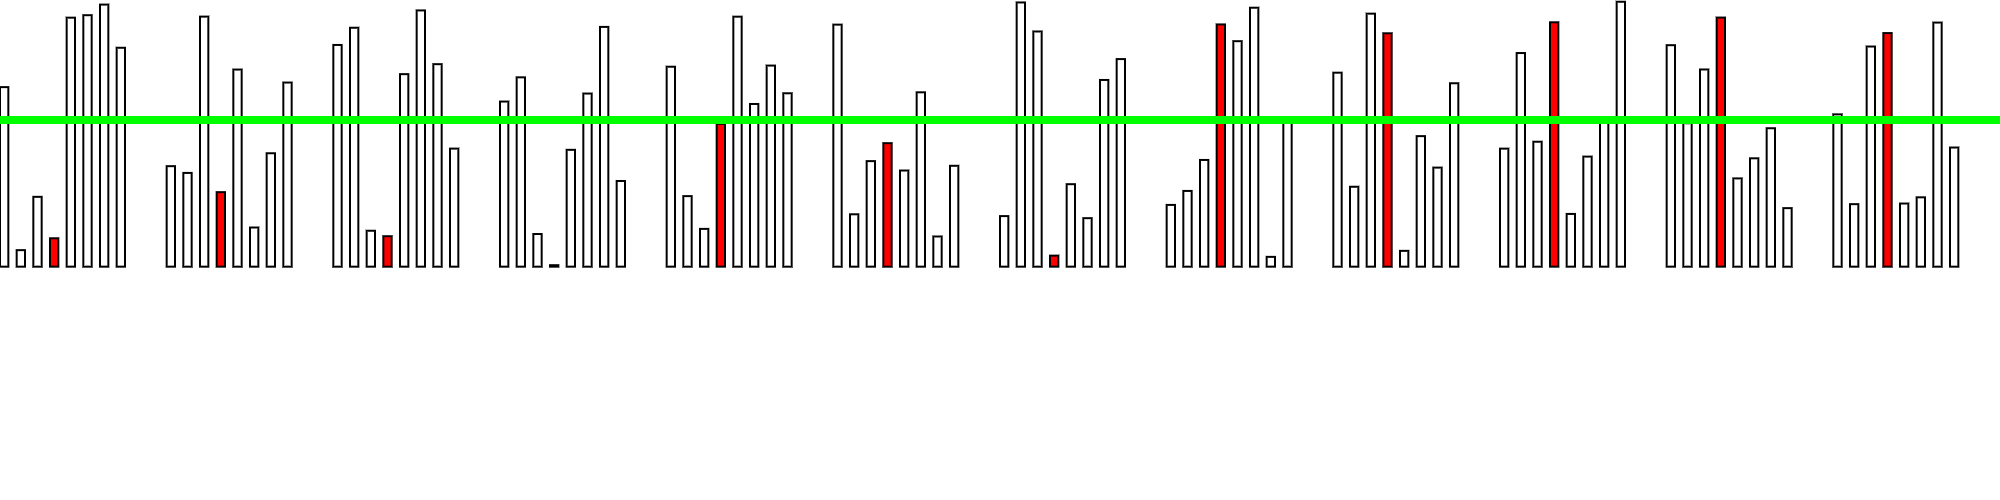
\includegraphics[width=\linewidth]{imgs/stridedAlgSim/stridedAlgSim_3.png}
	\onslide<4>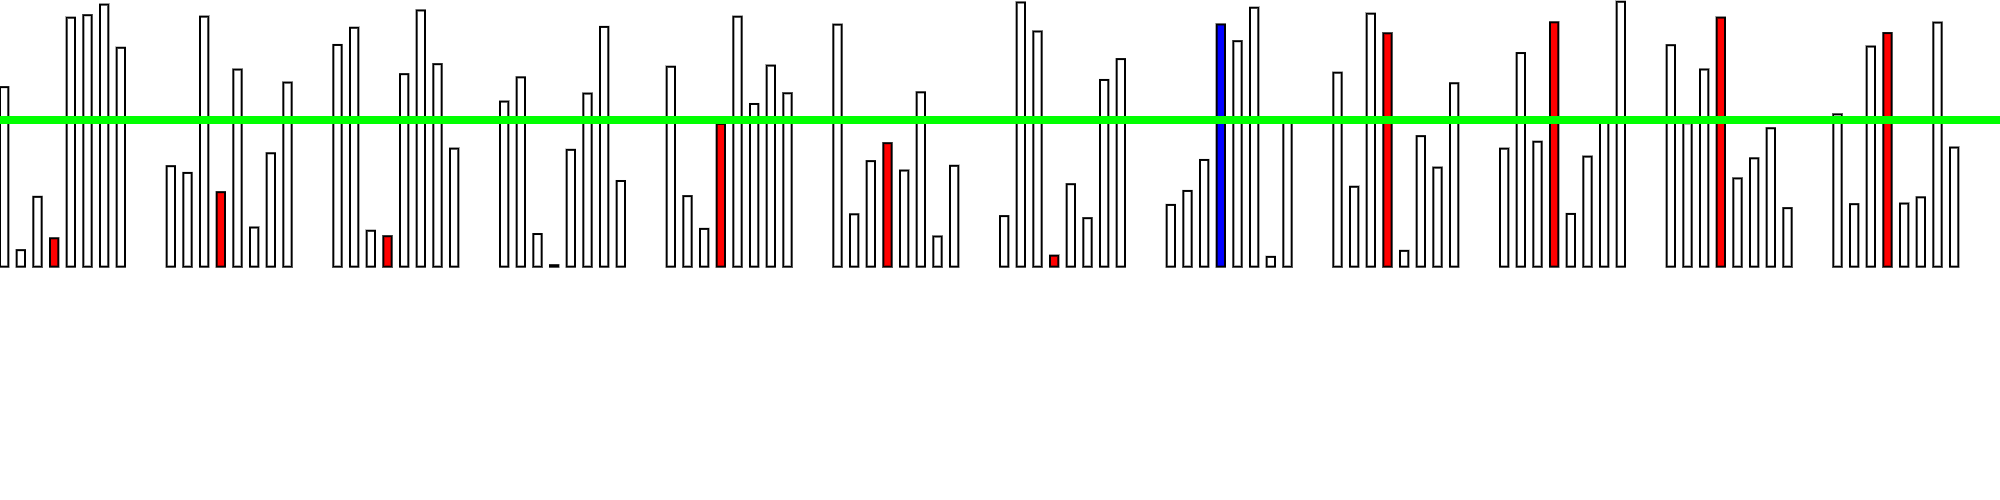
\includegraphics[width=\linewidth]{imgs/stridedAlgSim/stridedAlgSim_35.png}
	\onslide<5>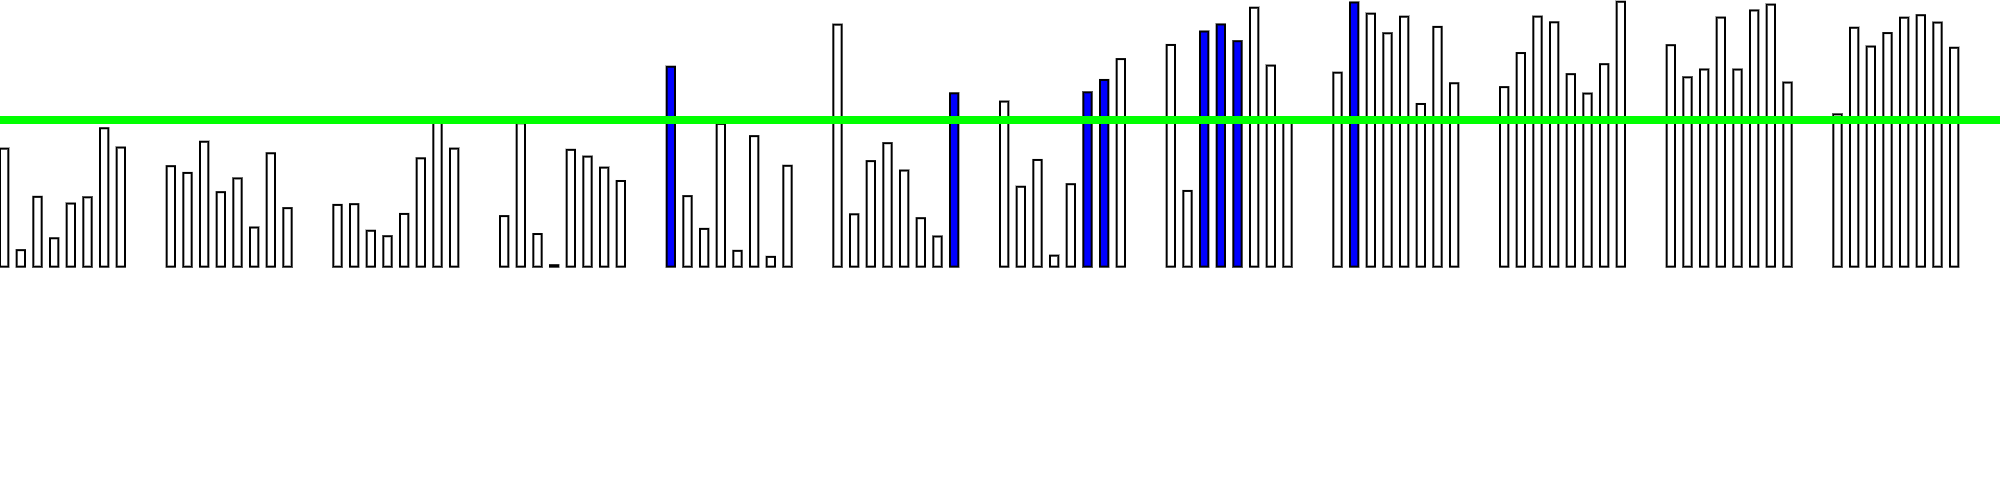
\includegraphics[width=\linewidth]{imgs/stridedAlgSim/stridedAlgSim_4.png}
	\onslide<6>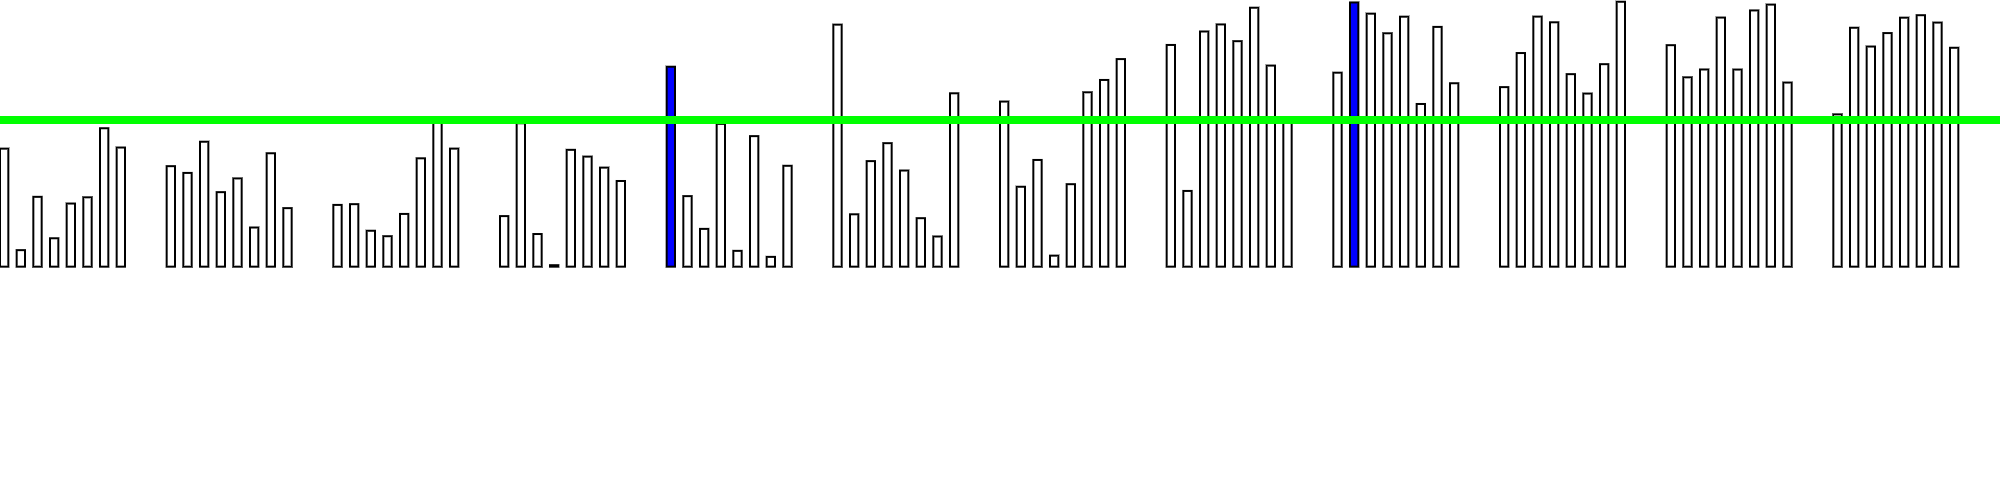
\includegraphics[width=\linewidth]{imgs/stridedAlgSim/stridedAlgSim_45.png}
	\onslide<7>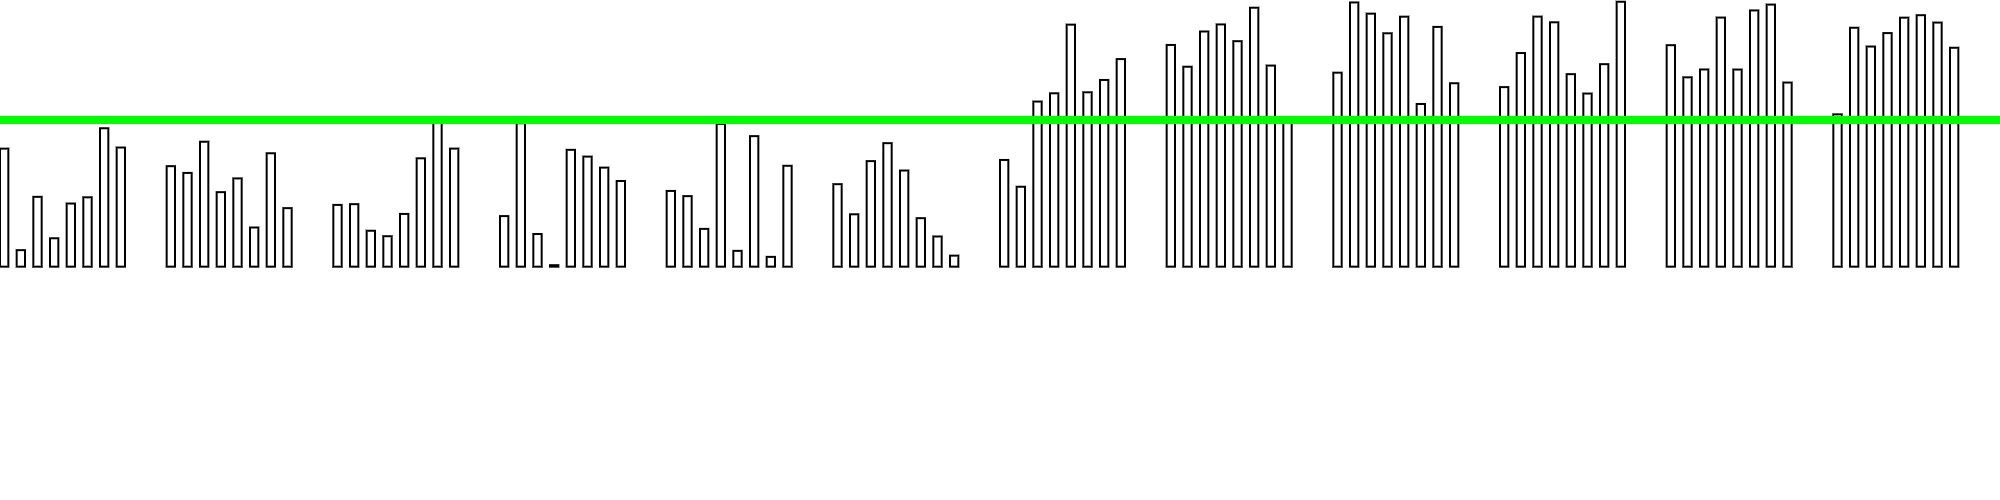
\includegraphics[width=\linewidth]{imgs/stridedAlgSim/stridedAlgSim_5.png}
	\end{overprint}
	\vspace{0.25cm}
	\begin{overprint}
	\onslide<3>This step is highly parallel.
	% \onslide<4>Note that all elements below the minimum splitting index are less than the pivot and all elements greater than the maximum splitting index are greater than the pivot.
	\onslide<7> Note that this step has no parallelism. In general this results in span $O(n)$. However, if the number of elements less than the pivot in each $P_i$ is similar, then size of the subarray to be partitioned can be very small.
	\end{overprint}
\end{frame}

% \begin{frame}[t]{Strided Algorithm Description [Francis and Pannan, 92; Frias and Petit, 08]}
%   % Partition $A$ into chunks $C_1,C_2,\ldots C_n/gb$ each consisting of $g$ cache lines of size $b$. Let $P_i$ be the union of the $i$-th cache-line from each chunk $C_j$.
%   \begin{figure}
%     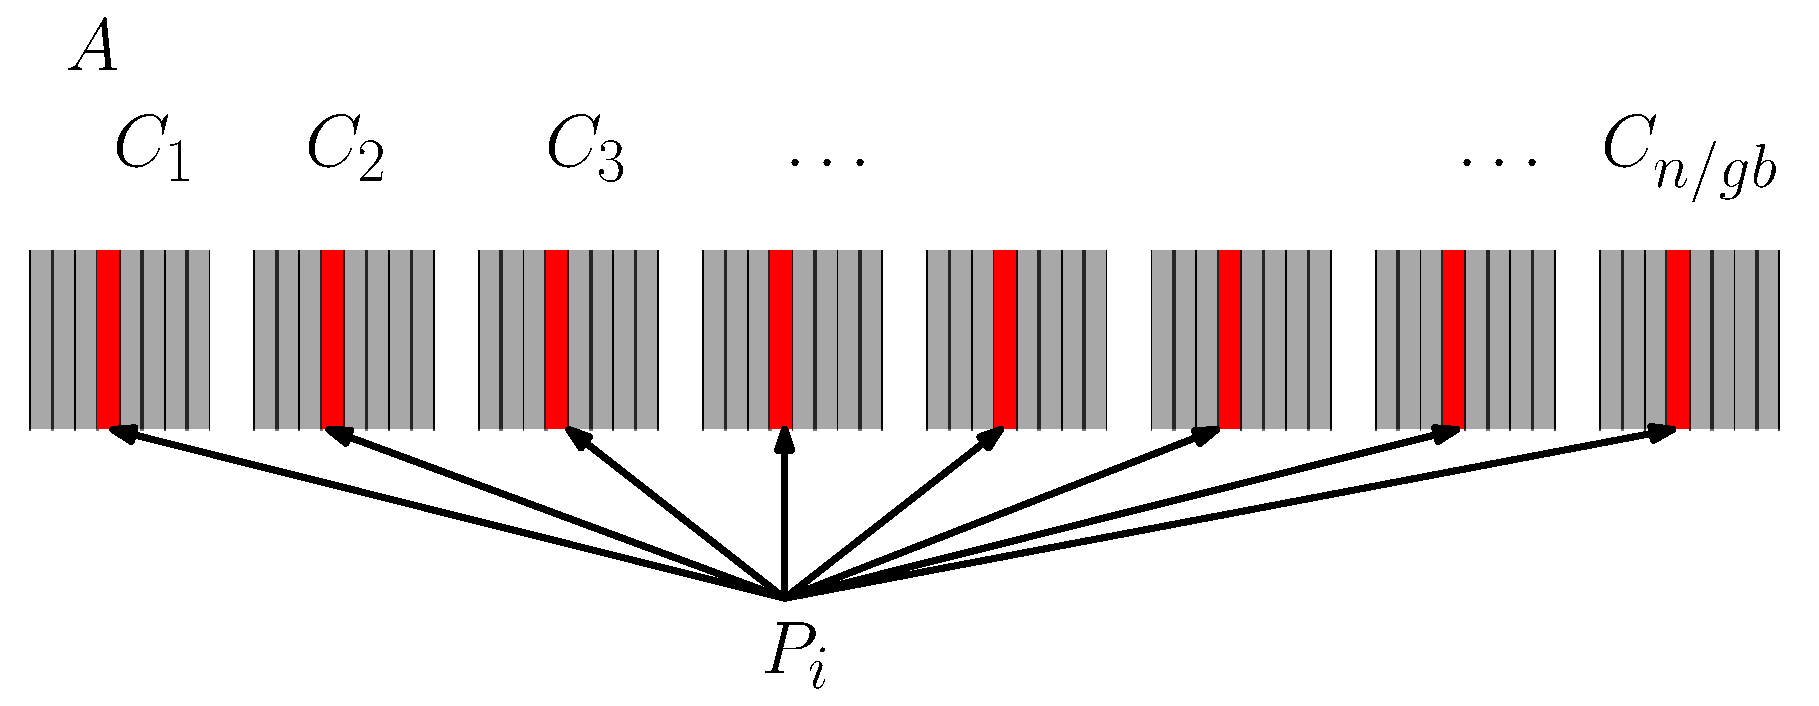
\includegraphics[width=\linewidth]{imgs/stridedAlgArrows.eps}
%   \end{figure}
%   % \begin{defin}[Partially Partitioned Array]
%   %   $\exists u, l $ such that $$i < u \implies A[i] \text{ is predecessor }, i \ge l \implies A[i] \text{ is successor }$$
%   % \end{defin}
%   \begin{itemize}
%     \item Logically partition $A_i$ into $P_i$ so that $P_i$ has the $i$-th block from each chunk $C_j$ of the array
%     \item Perform serial partitions on all $P_i$ in parallel.
%     \item Let $v_i$ be the position in $A$ of the first successor in $P_i$. Perform a serial partition on $A[\min_i v_i], \ldots, A[\max_i v_i -1]$.
%   \end{itemize}
% \end{frame}


% \begin{frame}[t]{Strided Algorithm Analysis}
%   \begin{itemize}
%     \item Partial partition step: work $O(n)$, span $\Theta(n/g)$.
%     \item Serial cleanup step: span $\Theta(v_\text{max}-v_\text{min})$, which is $O(n)$ in general.
%     \item If the number of predecessors in each $P_i$ is similar, $v_\text{max}-v_\text{min}$ can be small.
%     \item If array values are selected independently at random from some distribution, for appropriate choice of parameters, with high probability in $n$, the Strided Algorithm achieves span $$\tilde{O}(n^{2/3}),$$ and the number of cache misses is fewer than $$\frac{n}{b}+\frac{\tilde{O}(n^{2/3})}{b}.$$
%     % \item In particular, if $b\in \polylog(n)$, and the array values are selected independently at random from some distribution, and $g$ is chosen to optimize span ($g=n^{1/3}$), then with high probability in $n$, $$v_\text{max}-v_\text{min} < \tilde{O}(n^{2/3}),$$ the span is $$\tilde{O}(n^{2/3}),$$ and the number of cache misses is fewer than $$\frac{n}{b}+\frac{\tilde{O}(n^{2/3})}{b}.$$
%   \end{itemize}
% \end{frame}

% \begin{frame}[t]{The Smoothed Striding Algorithm} 
%   The Smoothed-Striding Algorithm creates groups analogous to the Strided Algorithm's $P_i$'s, but rather than taking the $i$-th element from each chunk of the array to form groups $P_i$, the Smoothed-Striding algorithm takes a random element from each chunk for each of the groups $U_i$.

%   \textbf{Blocked Strided Algorithm $P_i$.}
%   \begin{figure}
%     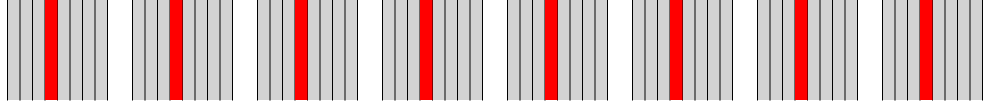
\includegraphics[width=\linewidth]{imgs/stridedAlgHighlighted.png}
%   \end{figure}
%   \textbf{Smoothed-Striding Algorithm $U_i$.}
%   \begin{figure}
%     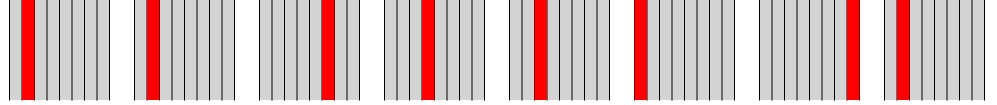
\includegraphics[width=\linewidth]{imgs/smoothedStridingAlgHighlighted.png}
%   \end{figure}
% \end{frame}


\begin{frame}[t]{}
	\vfill
	\begin{center}
		{\Huge The Smoothed-Striding Algorithm}
	\end{center}
	\vfill
\end{frame}

\begin{frame}[t]{}%{Smoothed Striding Algorithm Description}
	\vspace{0.25cm}
	\begin{overprint}
	\onslide<1>Logically partition the array into chunks of adjacent elements:
	\onslide<2>Form groups $U_i$ where $U_i$ contains the $i$-th element from each chunk:
	\onslide<3>Perform serial partitions on each $U_i$ in parallel over the $U_i$'s:
	\onslide<4>Identify the splitting index $v_i$ (the first element greater than the pivot) of each $P_i$. 
	\onslide<5>Recursively apply this algorithm to partition the subarray from the minimum splitting index to the maximum splitting index in serial. This completes the partition. 
	\end{overprint}
	\vspace{0.25cm}
	\begin{overprint}
	\onslide<1>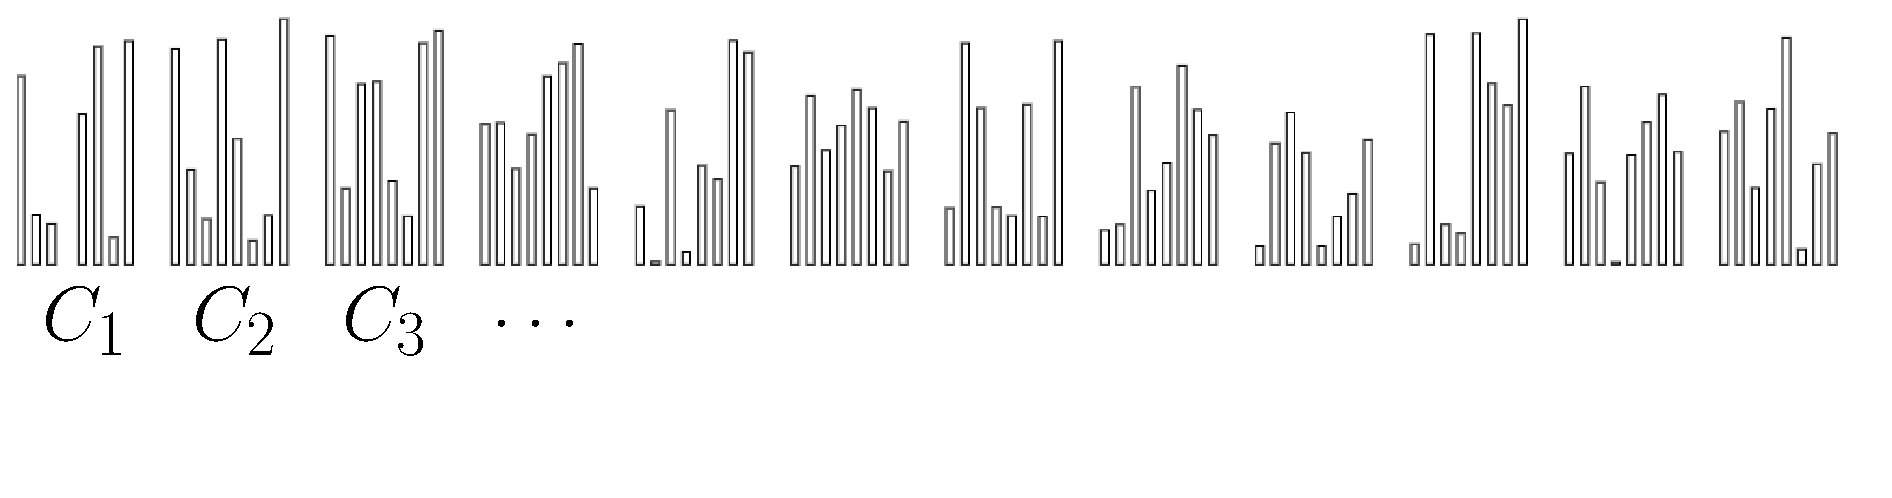
\includegraphics[width=\linewidth]{imgs/smoothedAlgSim1Ann.eps}
	\onslide<2>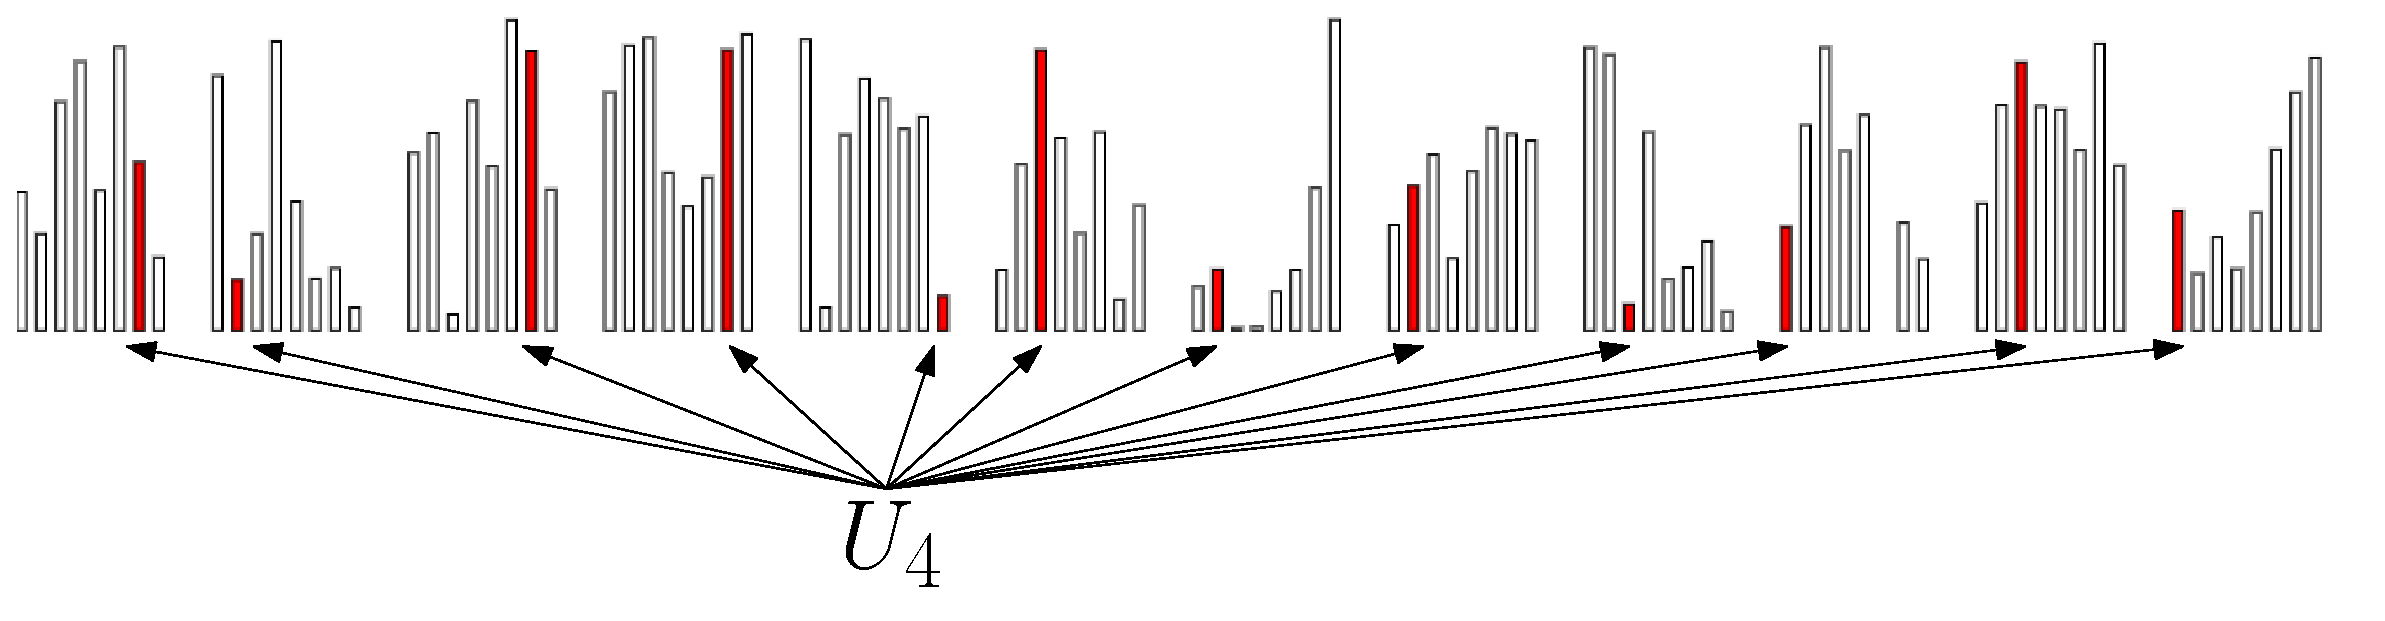
\includegraphics[width=\linewidth]{imgs/smoothedAlgSim2Ann.eps}
	\onslide<3>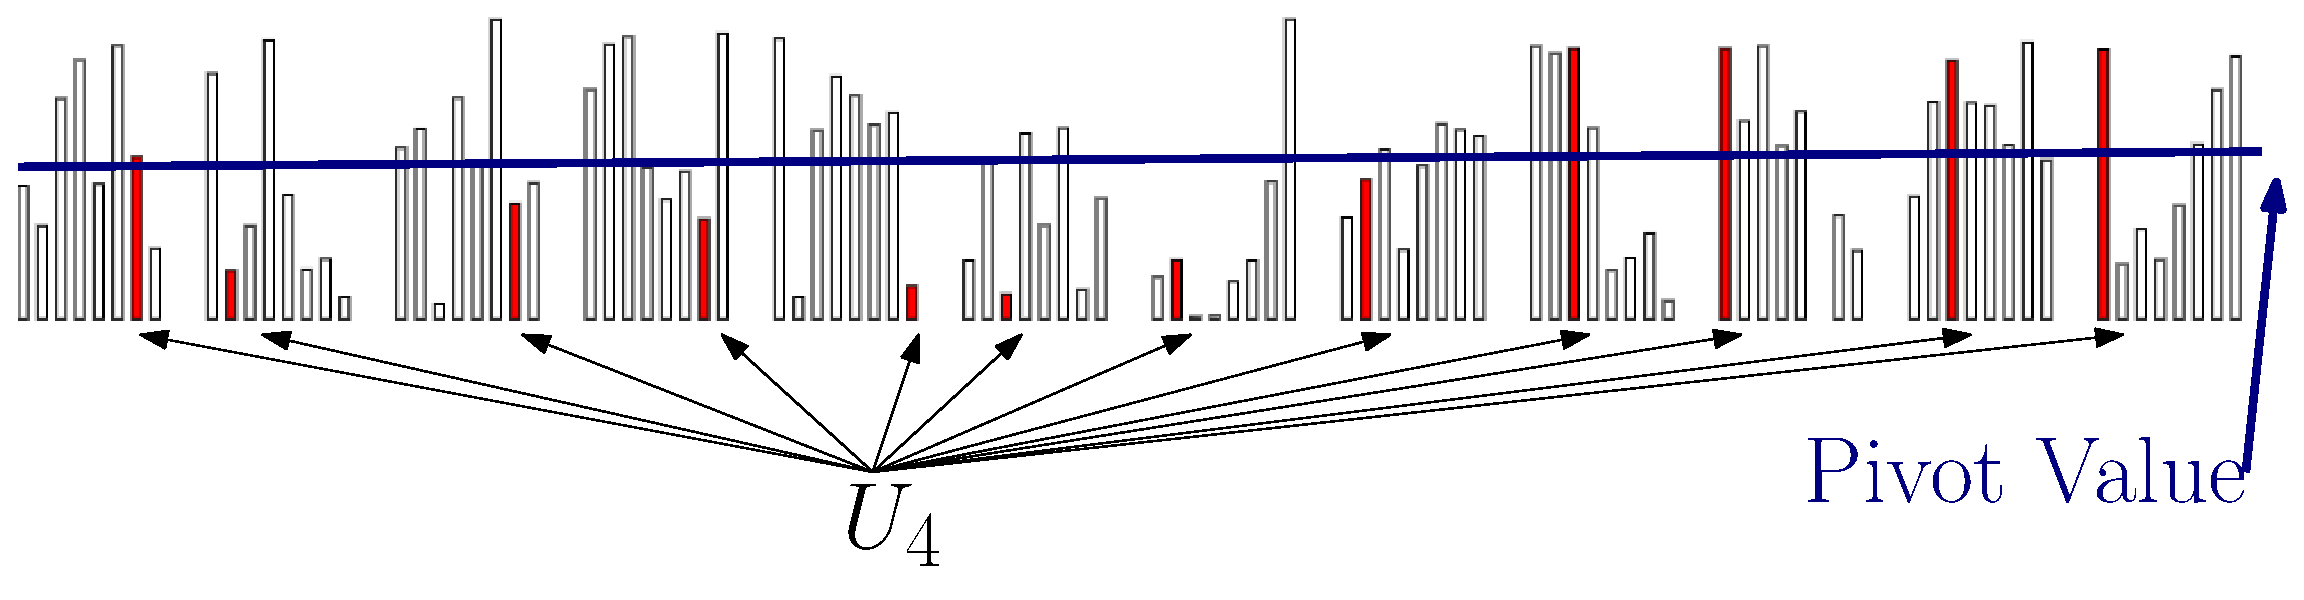
\includegraphics[width=\linewidth]{imgs/smoothedAlgSim3Ann.eps}
	\onslide<4>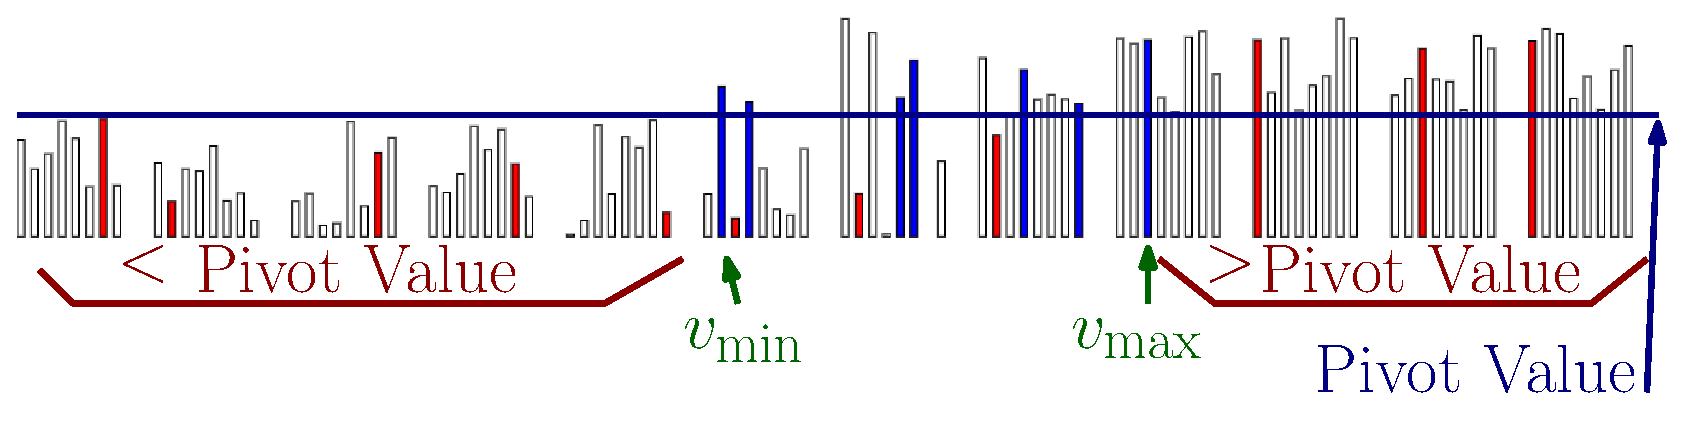
\includegraphics[width=\linewidth]{imgs/smoothedAlgSim4Ann.eps}
	\onslide<5>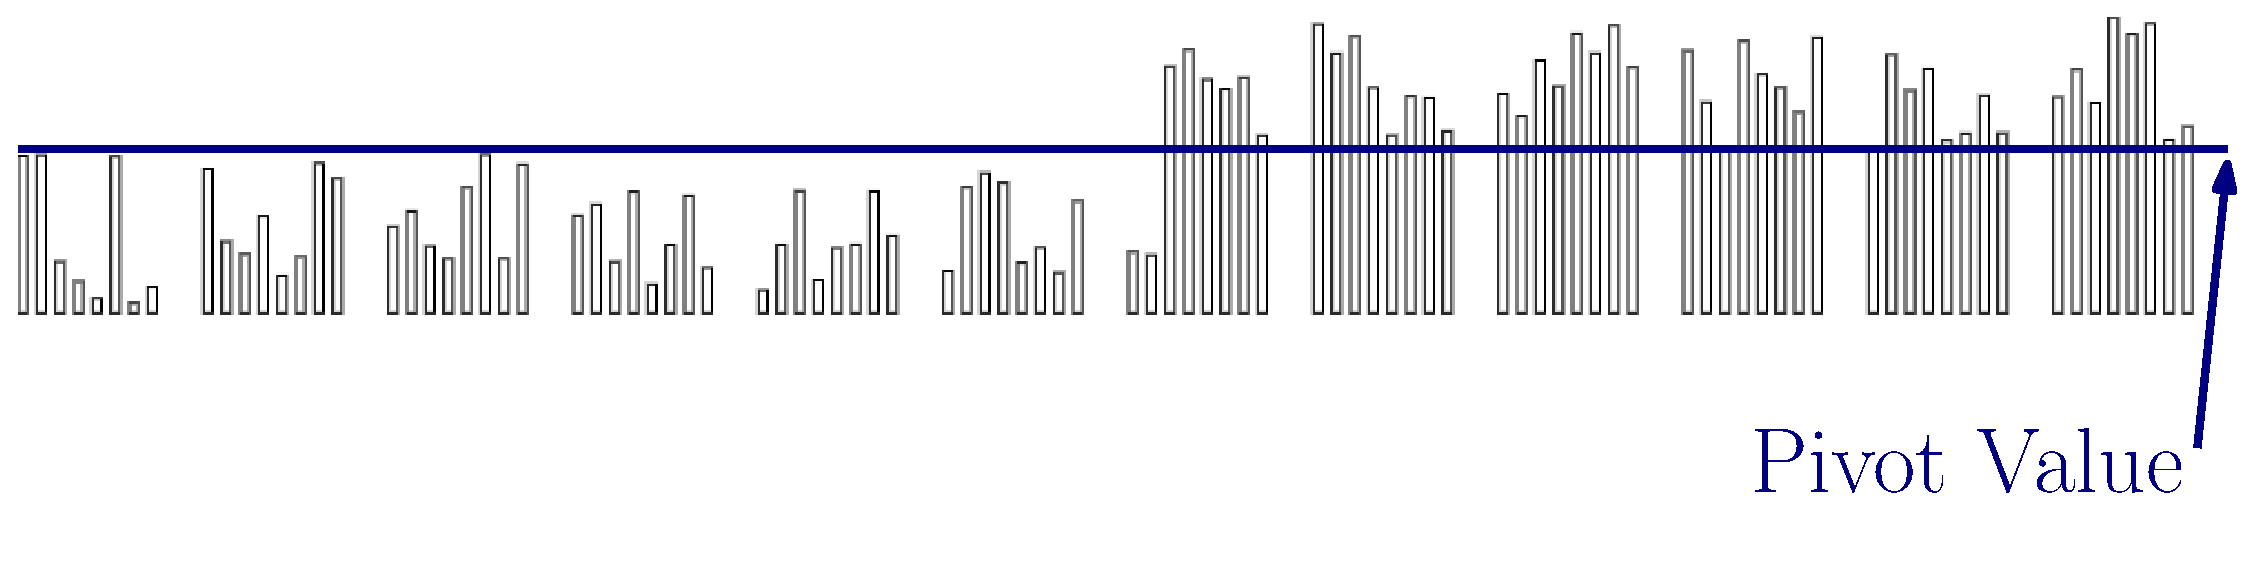
\includegraphics[width=\linewidth]{imgs/smoothedAlgSim5Ann.eps}
	\end{overprint}
	\vspace{0.25cm}
	\begin{overprint}
	\onslide<3>This step is highly parallel.
	% \onslide<4>Note that all elements below the minimum splitting index are less than the pivot and all elements greater than the maximum splitting index are greater than the pivot.
	\onslide<5>Unlike in the Strided Algorithm this step has parallelism, and is guaranteed to only run on a small subarray. The Strided Algorithm could not recurse here because the subproblem is a worst case input for it.
	\end{overprint}
\end{frame}

\begin{frame}[t]{}%{Smoothed Striding Algorithm Description}
	\vspace{0.25cm}
	\begin{overprint}
	\onslide<1>Logically partition the array into chunks of adjacent elements:
	\onslide<2>Form groups $U_i$ where $U_i$ contains the $i$-th element from each chunk:
	\onslide<3>Perform serial partitions on each $U_i$ in parallel over the $U_i$'s:
	\onslide<4>Identify the splitting index $v_i$ (the first element greater than the pivot) of each $P_i$. 
	\onslide<5>Recursively apply this algorithm to partition the subarray from the minimum splitting index to the maximum splitting index in serial. This completes the partition. 
	\end{overprint}
	\vspace{0.25cm}
	\begin{overprint}
	\onslide<1>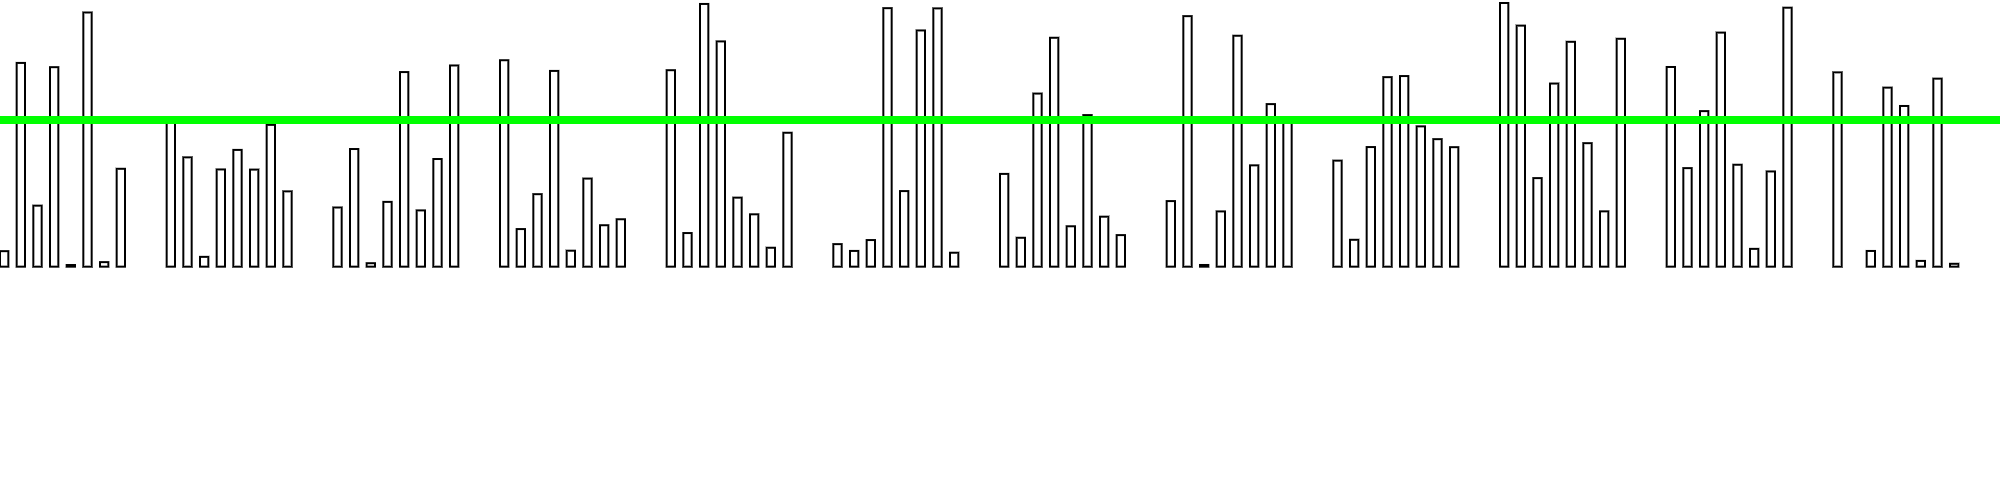
\includegraphics[width=\linewidth]{imgs/smoothedAlgSim/smoothedAlgSim_1.png}
	\onslide<2>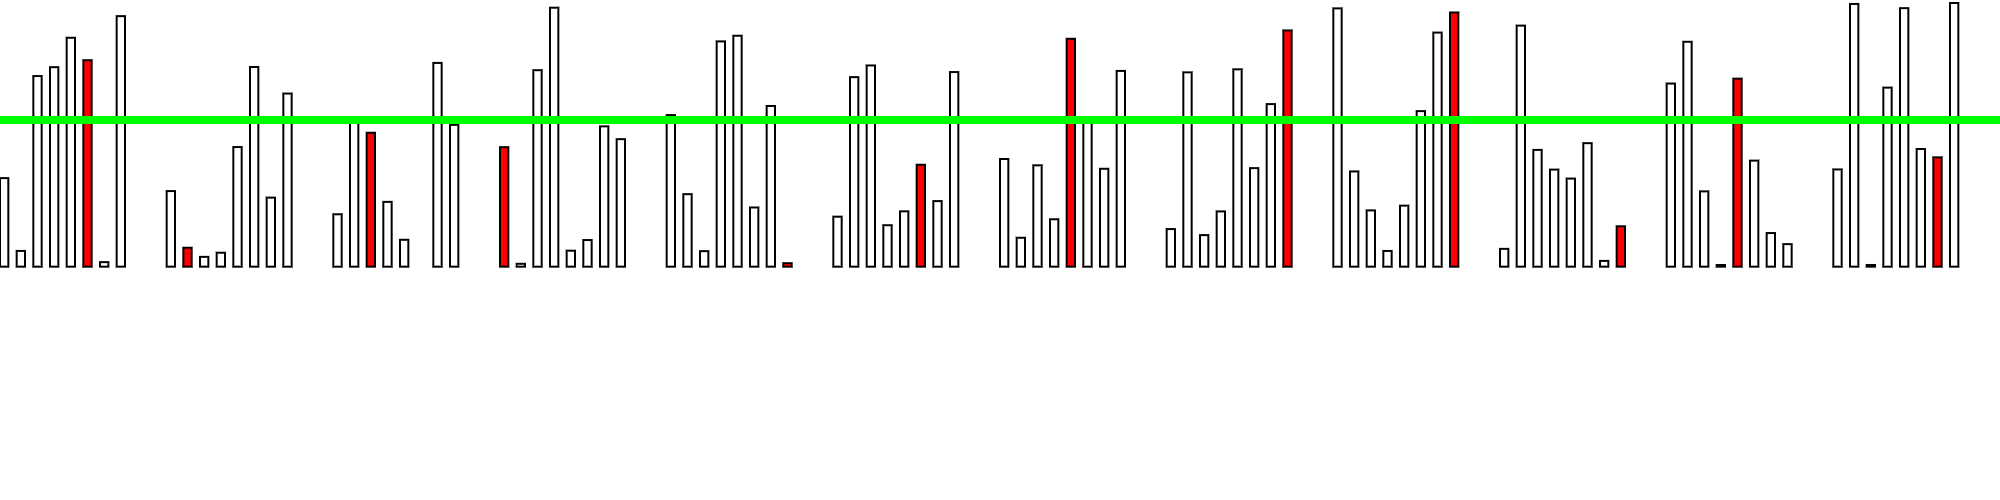
\includegraphics[width=\linewidth]{imgs/smoothedAlgSim/smoothedAlgSim_2.png}
	\onslide<3>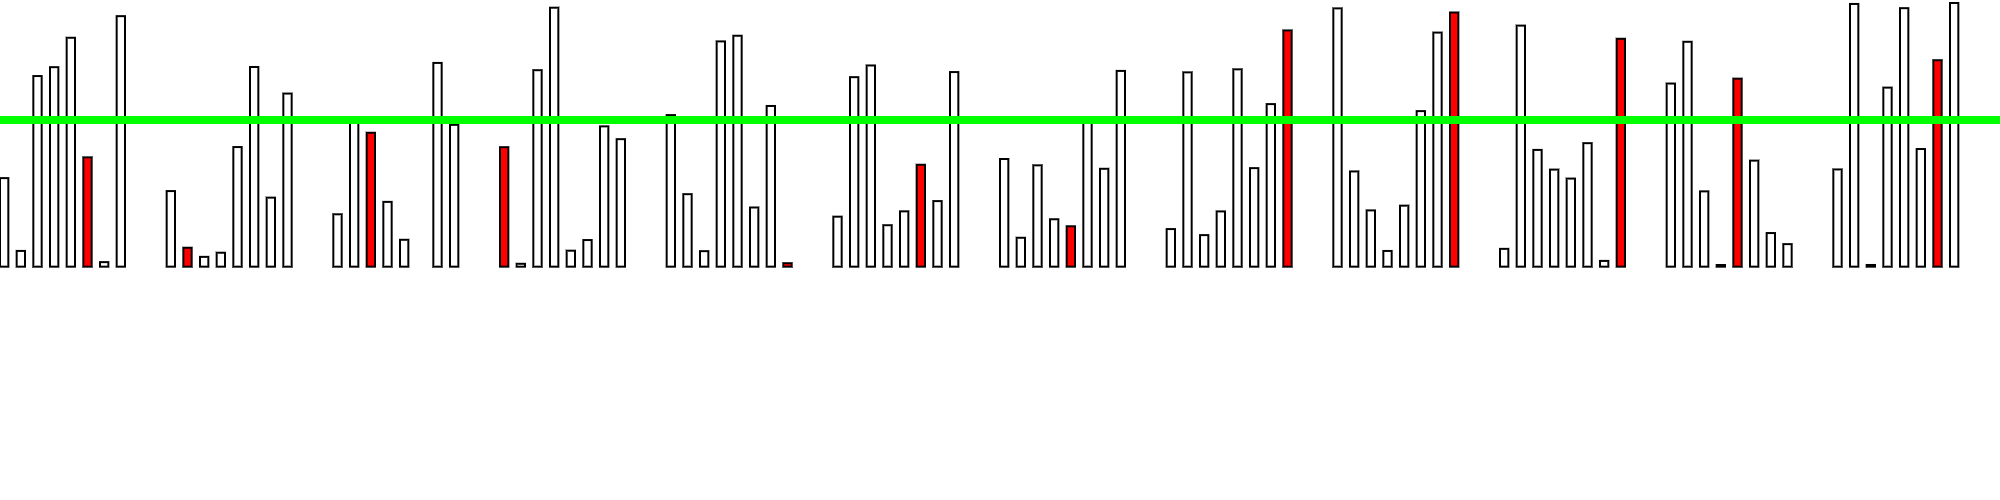
\includegraphics[width=\linewidth]{imgs/smoothedAlgSim/smoothedAlgSim_3.png}
	\onslide<4>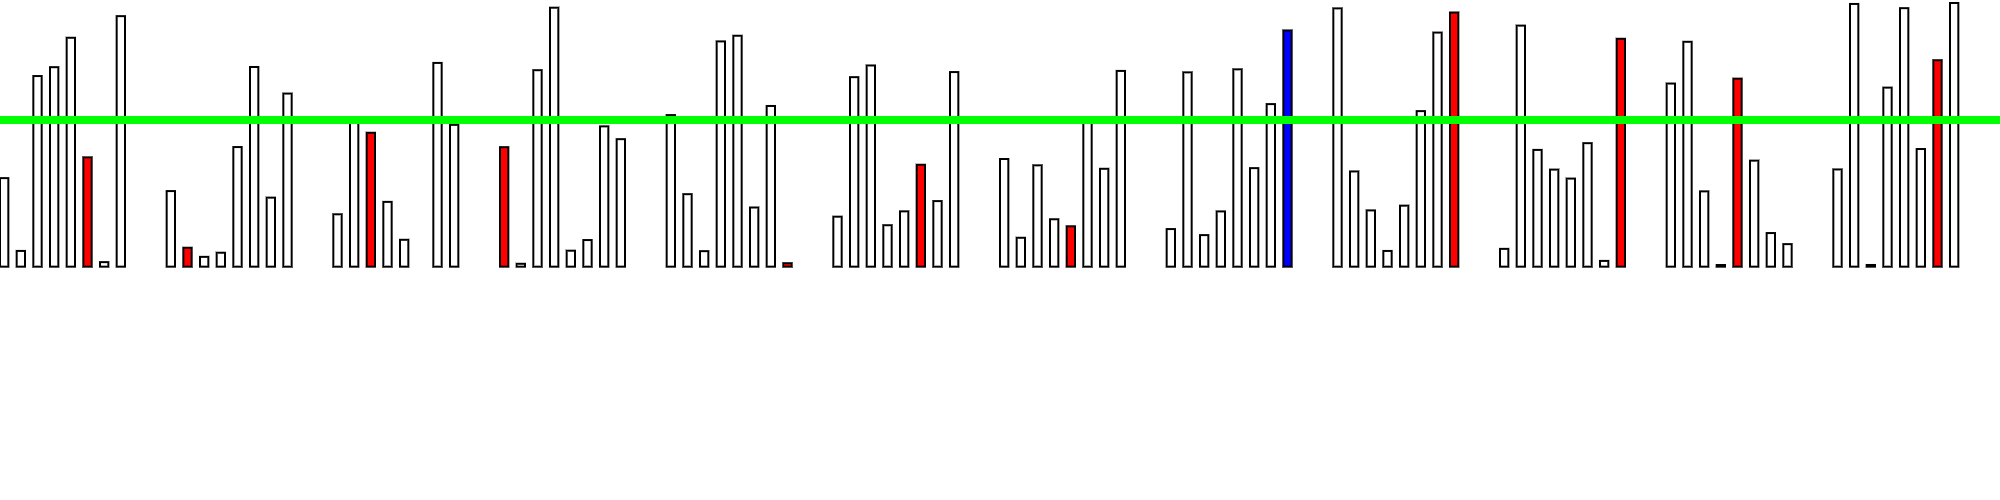
\includegraphics[width=\linewidth]{imgs/smoothedAlgSim/smoothedAlgSim_35.png}
	\onslide<5>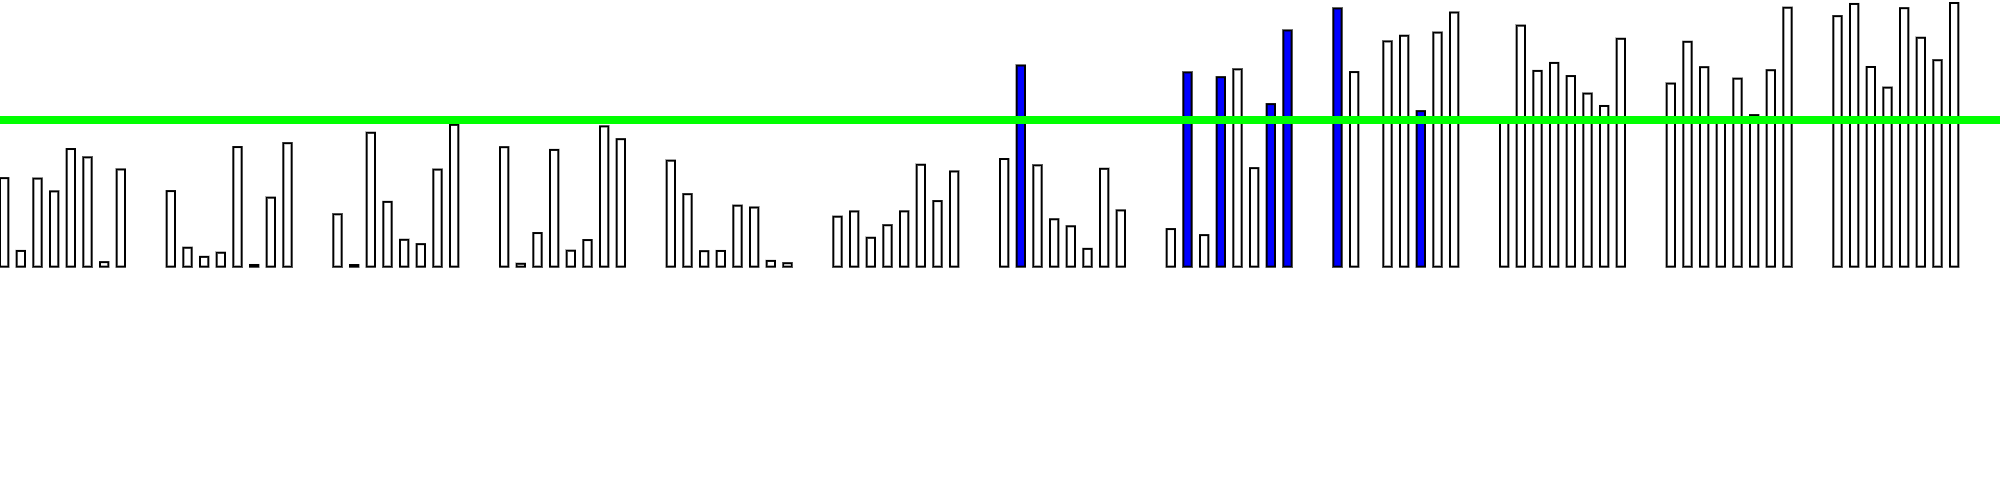
\includegraphics[width=\linewidth]{imgs/smoothedAlgSim/smoothedAlgSim_4.png}
	\onslide<6>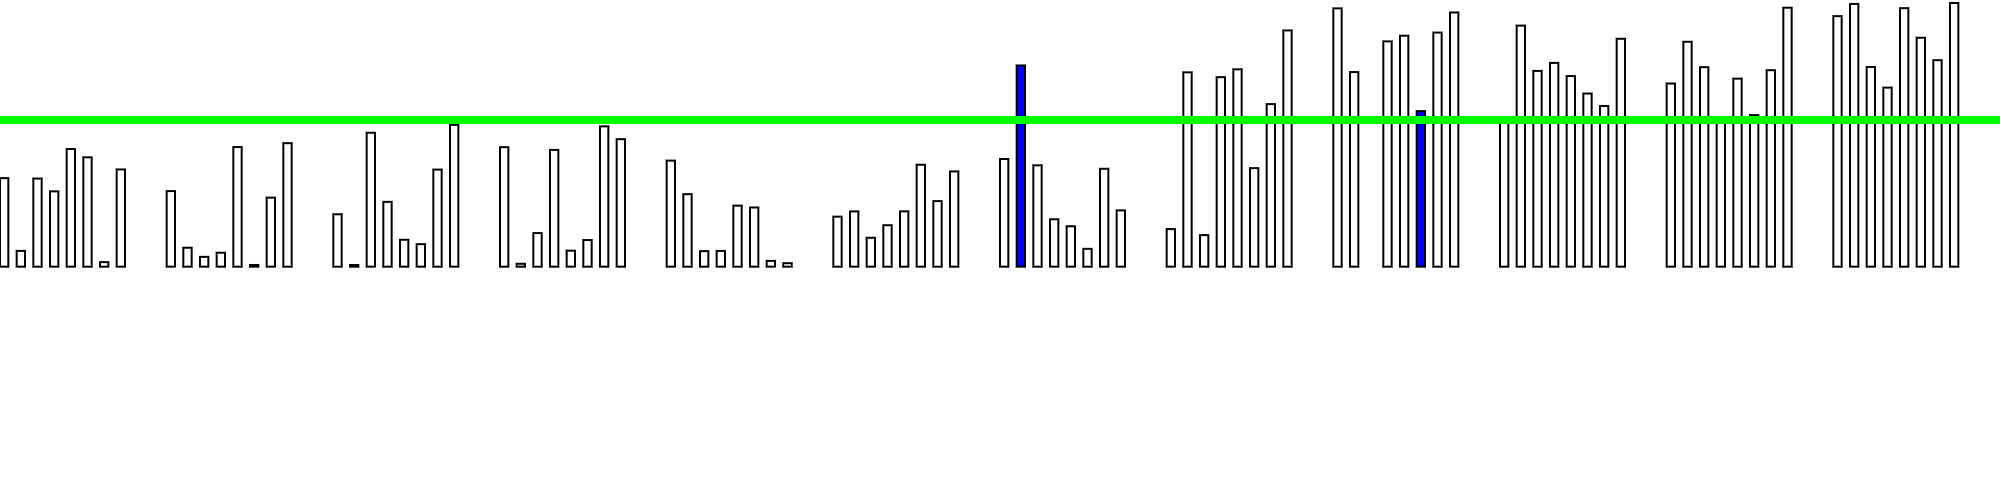
\includegraphics[width=\linewidth]{imgs/smoothedAlgSim/smoothedAlgSim_45.png}
	\onslide<7>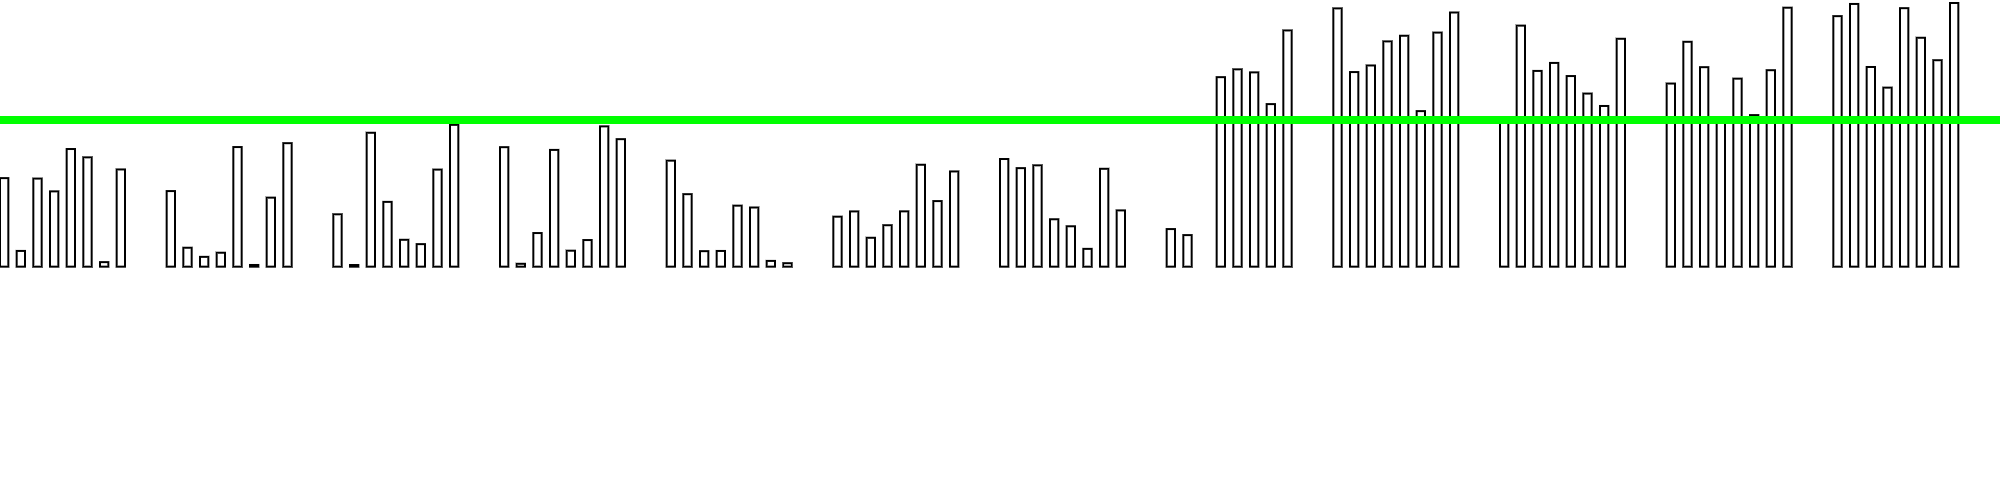
\includegraphics[width=\linewidth]{imgs/smoothedAlgSim/smoothedAlgSim_5.png}
	\end{overprint}
	\vspace{0.25cm}
	\begin{overprint}
	\onslide<3>This step is highly parallel.
	% \onslide<4>Note that all elements below the minimum splitting index are less than the pivot and all elements greater than the maximum splitting index are greater than the pivot.
	\onslide<7>Unlike in the Strided Algorithm this step has parallelism, and is guaranteed to only run on a small subarray. The Strided Algorithm could not recurse here because the subproblem is a worst case input for it.
	\end{overprint}
\end{frame}

% \begin{frame}[t]{Technical Notes}
%   Storing the groups $U_i$ is a challenge. We can't explicitly store them because then the algorithm would not be in-place. By design they do not have a regular structure like the $P_i$ of the Strided Algorithm.\\
%   The solution is to store $U_1$ and then specify that all other $U_i$'s are a circular shift within the chunks of $U_1$.\\
%   More precisely, Let $X[1],\ldots, X[s]$ be chosen uniformly at random from $\{1,\ldots, g\}$. 
%   Then let $U_i$ be the union of the $(X[j]+i)\mod g$-th cache-line from each chunk $C_j$.\\
%   Note that the $U_i$'s are not indpendent, but this doesn't affect the union bound.\\
%   \vspace{0.5cm}
%   In order to compute the minimum and maxmium splitting indices $v_{\min}, v_{\max}$ in parallel we use a recursive structure rather than a parallel-for loop.
% \end{frame}

\begin{frame}[t]{A Key Challenge}
How do we store the $U_i$'s if they are all random?	\\
\vspace{0.5cm}
If we stored the parts that made up each $U_i$ we would not be in-place.\\
\vspace{0.5cm}
\textbf{Blocked Strided Algorithm $P_i$.}
\begin{figure}
	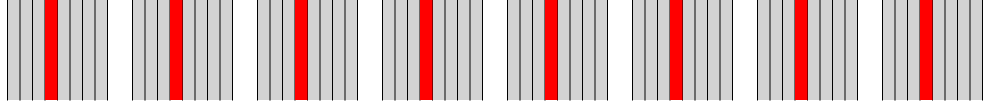
\includegraphics[width=\linewidth]{imgs/stridedAlgHighlighted.png}
\end{figure}
\textbf{Smoothed-Striding Algorithm $U_i$.}
\begin{figure}
	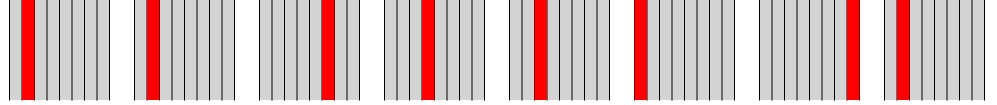
\includegraphics[width=\linewidth]{imgs/smoothedStridingAlgHighlighted.png}
\end{figure}
\end{frame}


% \begin{frame}[t]{Smoothed Striding Algorithm Description}
%   Let $X[1],\ldots, X[s]$ be chosen uniformly at random from $\{1,\ldots, g\}$. Let $U_i$ be the union of the $(X[j]+i)\mod g$-th cache-line from each chunk $C_j$.
%   \begin{figure}
%     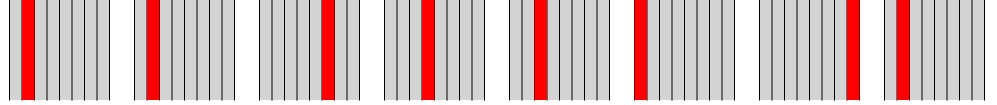
\includegraphics[width=\linewidth]{imgs/smoothedStridingAlgHighlighted.png}
%   \end{figure}
%   \begin{itemize}
%     \item Perform serial partitions on all $U_i$ in parallel.
%     \item The array is partially now partitioned with $A[i]$ a predecessor for all $i < v_{\text{min}}$ and $A[i]$ a successor for all $i \ge v_{\text{max}}$.
%   \end{itemize}
%   Note that we will make $s = \frac{n}{gb} < \polylog(n)$ so the algorithm remains in-place.
% \end{frame}


% \begin{frame}[t]{Partial Partition Step Analysis}
% \begin{proposition}
%   %% The 1/2's are necessary for the final line of the proof to easily go through.
%   Let $\epsilon \in (0, 1/2)$ and $\delta \in (0, 1/2)$ such that
%   $\epsilon \ge \frac{1}{\poly(n)}$ and $\delta \ge
%   \frac{1}{\polylog(n)}$. Suppose $s > \frac{\ln
%     (n/\epsilon)}{\delta^2}$. Finally, suppose that each processor has
%   a cache of size at least $s + c$ for a sufficiently large constant
%   $c$.

%   Then the Partial-Partition Algorithm achieves work $O(n)$; achieves
%   span $O\paren*{b \cdot s}$; incurs $\frac{s+n}{b} + O(1)$ cache
%   misses; and guarantees with probability $1 - \epsilon$ that
%   $$v_{\text{max}}-v_{\text{min}} < 4 n \delta.$$
% \end{proposition}

% \end{frame}

% \begin{frame}[t]{From Partial Partition to Full Partition}
%   \emph{Partial Partition Step:}
%   \begin{itemize}
%     \item Use $\epsilon = 1/n^c$ for $c$ of our choice (i.e. with high probability).
%     \item Choice of $\delta$ results in tradeoff between cache misses and span.
%   \end{itemize}
% \end{frame}

% \begin{frame}[t]{From Partial Partition to Full Partition}
%   \emph{Recursive strategies:}
%   \begin{itemize}
%     \item \defn{Hybrid Smoothed Striding Algorithm}: Use algorithm with span $O(\log n \log \log n)$. Note: recursive algorithm's cache behavior doesn't affect overall cache behavior because subarray is small. This algorithm can be tuned to give optimal span and cache misses.
%     \item \defn{Recursive Smoothed Striding Algorithm}: Use the Partial Partition step recursively to solve subproblems. Recursive applications of the Partial Partition step use the same $\epsilon$ the top-level (to guarantee success with high probability in $n$), and use $\delta \in \Theta(1)$ such that the problem size is reduced by half at each step. This algorithm has slightly worse span, but is very simple to implement.
%   \end{itemize}
% \end{frame}

% \begin{frame}[t]{Hybrid Algorithm Analysis - General Theorem}
% \begin{theorem}
%   The Hybrid Smoothed Striding Algorithm algorithm using parameter $\delta\in(0,1/2)$ satisfying $\delta \ge 1/\polylog(n)$: has work $O(n)$; achieves span
%         $$O\paren*{\log n \log\log n +\frac{b\log n}{\delta^2}},$$
% with high probability in $n$; and incurs fewer than 
% $$(n+O(n\delta))/b$$
% cache misses with high probability in $n$.
% \end{theorem}
% \end{frame}

% \begin{frame}[t]{Hybrid Algorithm Analysis - Corollary for specific parameter settings}
% An interesting corollary of the above theorem concerns what happens when $b$ is small (e.g., constant) and we choose $\delta$ to optimize span. 
% \begin{corollary}
% Suppose $b \le o(\log \log n)$. Then the Cache-Efficient Full-Partition Algorithm algorithm using $\delta = \Theta\big(\sqrt{b/\log\log n}\big)$, achieves work $O(n)$, and with high probability in $n$, achieves span $O(\log n \log\log n)$ and incurs fewer than $(n+o(n))/b$ cache misses.
% \end{corollary}
% \end{frame}


% \begin{frame}[t]{Recursive Algorithm Analysis - General Theorem}
%   \begin{theorem}
%   With high probability in $n$, the Recursive Smoothed Striding
%         algorithm using parameter $\delta \in(0,1/2)$ satisfying
%         $\delta \ge 1 / \polylog(n)$: achieves work $O(n)$, attains span
%   $$O\left(b\left(\log^2 n + \frac{\log n}{\delta^2}\right)\right),$$
%   and incurs $(n+O(n \delta))/b$ cache misses. 
%   \end{theorem}
% \end{frame}

% \begin{frame}[t]{Recursive Algorithm Analysis - Corollary for specific parameter settings}
% A particularly natural parameter setting for the Recursive algorithm occurs at $\delta = 1 / \sqrt{\log n}$.
% \begin{corollary}
%   With high probability in $n$, the Recursive Smoothed Striding Algorithm using parameter $\delta=1/\sqrt{\log n}$:
%   achieves work $O(n)$, attains span $O(b\log^2 n)$, and incurs $n/b \cdot (1 + O(1 / \sqrt{\log n}))$ cache misses. 
% \end{corollary}
% \end{frame}


\begin{frame}[t]{Open Questions}
	By recursively applying the Smoothed-Striding algorithm we get an algorithm for
	parallel partition that incurs $n(1+o(1))$ cache misses and has span
	$O(b\log^2 n)$.\\
	\vspace{0.25cm}
	There are techniques for improving this span to $O(\log n\log\log n)$ while retaining the cache behavior.\\
	\vspace{0.25cm}
	But the standard algorithm has span $O(\log n)$.\\
	\vspace{1cm}
	Can we construct an algorithm that achieves optimal cache behavior and span $O(\log n)$?
\end{frame}

\begin{frame}[t]{Acknowledgments}
I would like to thank
\begin{itemize}
	\item {The MIT PRIMES program}
	\item {William Kuszmaul, my PRIMES mentor}
	\item {My parents}
\end{itemize}
\end{frame}

\end{document}
